%%%%%%%%%%%%%%%%%%%%%%%%%%%%%%%%%%%%%%%%%
% 6-DOF Robotic Arm - Project Report
%%%%%%%%%%%%%%%%%%%%%%%%%%%%%%%%%%%%%%%%%

\documentclass[12pt,a4paper]{report}

% Basic packages
\usepackage[utf8]{inputenc}
\usepackage[T1]{fontenc}
\usepackage{lmodern}
\usepackage[english]{babel}
\usepackage{geometry}
\geometry{margin=2.5cm}

% Graphics
\usepackage{graphicx}
\usepackage{float}

% Tables
\usepackage{booktabs}
\usepackage{tabularx}

% Code listings
\usepackage{listings}
\usepackage{xcolor}

% Math
\usepackage{amsmath}
\usepackage{amssymb}

% TikZ for diagrams
\usepackage{tikz}
\usetikzlibrary{shapes,arrows,positioning,fit}

% Hyperlinks
\usepackage{hyperref}
\hypersetup{colorlinks=true, linkcolor=blue!60!black}

% Code style
\lstset{
    basicstyle=\ttfamily\small,
    breaklines=true,
    frame=single,
    backgroundcolor=\color{gray!10}
}

%% ========================================
%% DOCUMENT INFO
%% ========================================

\title{
    \vspace{2cm}
    {\Huge\bfseries Design and Implementation of a}\\[0.3cm]
    {\Huge\bfseries 6-DOF Robotic Manipulator}\\[0.5cm]
    {\Huge\bfseries with Singularity-Robust Motion Control}\\[0.8cm]
    {\LARGE Project Report}\\
    \vspace{2cm}
}

\author{
    Anwesh Rijal (16940572) \\
    Austin Matthew \\
    \textit{Hochschule Ravensburg-Weingarten University}
}

\date{
    January 2026
}

%% ========================================
%% DOCUMENT
%% ========================================

\begin{document}

% Title page
\maketitle
\thispagestyle{empty}
\newpage

% Table of contents
\tableofcontents
\newpage

%% ========================================
%% PART 1: INTRODUCTION
%% ========================================

\chapter{Introduction}

\section{Project Background}

This project involves the development of a 6-DOF robotic arm control system, including custom firmware and host software. The mechanical design is based on the open-source \textbf{PAROL6} desktop robot arm developed by Source Robotics.

\subsection{Base Design Attribution}

The robot hardware design used in this project is derived from:

\begin{itemize}
    \item \textbf{PAROL6 Desktop Robot Arm} by Source Robotics
    \item Design by Petar Crnjak (\url{https://github.com/PCrnjak})
    \item Documentation: \url{https://source-robotics.github.io/PAROL-docs/}
    \item Hardware: \url{https://github.com/PCrnjak/PAROL6-Desktop-robot-arm}
\end{itemize}

This project extends the base PAROL6 design with custom firmware and software implementations.

\section{Project Objectives}

The primary objectives of this project are:

\begin{enumerate}
    \item \textbf{Build a Fully Functional 6-DOF Robotic Arm}: Assemble and integrate the mechanical structure, stepper motors, control electronics, and end effector into a working desktop manipulator.
    
    \item \textbf{Develop Stable Motion Control Software}: Implement a robust inverse kinematics controller capable of smooth, singularity-free motion throughout the workspace.
    
    \item \textbf{Implement Real-Time Control}: Create firmware and host software that can execute motion commands with low latency and high precision.
\end{enumerate}

\subsection{Controller Objectives}

The motion controller specifically aims to:
\begin{itemize}
    \item Provide stable velocity-level IK using quadratic programming (QP)
    \item Handle kinematic singularities gracefully using adaptive damping
    \item Support real-time interactive control via visualization interface
    \item Respect joint position and velocity limits at all times
\end{itemize}

\subsection{Software Architecture}

The control software consists of two main components:

\begin{itemize}
    \item \textbf{MCU Firmware} (STM32F446): Handles low-level motor control, step generation, S-curve motion profiles, and serial communication with the host.
    
    \item \textbf{Host Software} (C++/Qt): Implements kinematics computation (FK/IK), the QP-based differential controller with singularity handling, and 3D visualization for interactive control.
\end{itemize}

\section{Scope}

This project covers:
\begin{itemize}
    \item Mechanical assembly of the PAROL6-based robot arm
    \item Custom control board with STM32F446 and TMC5160 drivers
    \item MCU firmware for motion execution
    \item Host-side kinematics and motion control software
    \item 3D visualization and user interface
\end{itemize}

\section{Document Structure}

\begin{itemize}
    \item \textbf{Chapter 2 - Hardware}: Robot mechanical design, control board, electrical connections
    \item \textbf{Chapter 3 - MCU Firmware}: Motor control, S-curve profiles, communication
    \item \textbf{Chapter 4 - Motion Control Software}: Kinematics, QP-based differential controller, visualization
    \item \textbf{Appendices}: Pinout, DH parameters, joint limits
\end{itemize}

%% ========================================
%% PART 2: HARDWARE
%% ========================================

\chapter{Hardware}

This chapter describes the physical hardware of the our robotic arm system.

%% --- Section 1: The Robot ---
\section{The Robot}

\subsection{Overview}

Our robot is based on the \textbf{PAROL6} open-source robot arm design by Source Robotics. It is a 6 degrees of freedom (6-DOF) desktop robotic arm designed for education, research, and light industrial applications. The robot features an articulated arm configuration with all revolute joints, providing full spatial manipulation capability.

The mechanical design, including 3D printed parts and assembly, follows the original PAROL6 specifications with modifications for this project.

\begin{table}[H]
    \centering
    \begin{tabular}{|l|l|}
        \hline
        \textbf{Parameter} & \textbf{Value} \\
        \hline
        Degrees of Freedom & 6 rotating joints \\
        Weight & 5.5 kg \\
        Power Consumption & 40 W \\
        Material & 3D printed ABS plastic \\
        Communication & USB \\
        \hline
    \end{tabular}
    \caption{Robot Specifications}
    \label{tab:robot_specs}
\end{table}

\subsection{Mechanical Structure}

The robot is constructed primarily from 3D printed ABS plastic. ABS provides good mechanical strength and thermal resistance for this application.

\subsubsection{Joint Configuration}

\begin{table}[H]
    \centering
    \begin{tabular}{|c|l|c|l|}
        \hline
        \textbf{Joint} & \textbf{Function} & \textbf{Range} & \textbf{Reduction} \\
        \hline
        J1 & Base rotation & 250° & Belt 6.4:1 \\
        J2 & Shoulder lift & 141° & Planetary 20:1 \\
        J3 & Elbow bend & 180° & Planetary 20:1 + Belt 38:42 \\
        J4 & Wrist rotation & 212° & Belt 4:1 \\
        J5 & Wrist pitch & 180° & Belt 4:1 \\
        J6 & Tool rotation & $\infty$ & Planetary 10:1 \\
        \hline
    \end{tabular}
    \caption{Joint Configuration and Reduction Ratios}
    \label{tab:joint_config}
\end{table}


\subsubsection{Spherical Wrist Design}

The robot uses a \textbf{spherical wrist} configuration, where the last three joint axes (J4, J5, J6) intersect at a single point called the wrist center. This design is common in industrial manipulators and simplifies inverse kinematics by decoupling position and orientation problems.

\subsubsection{Kinematic Singularities}

Singularities are configurations where the robot loses one or more degrees of freedom. For our 6-DOF spherical wrist arm, three main singularities exist:

\begin{enumerate}
    \item \textbf{Wrist Singularity}: Occurs when J4 and J6 axes align (J5 = 0° or 180°)
    \item \textbf{Shoulder Singularity}: Wrist center lies on the J1 axis
    \item \textbf{Elbow Singularity}: Arm fully extended or folded
\end{enumerate}

Near singularities, the inverse Jacobian produces very large joint velocities, causing instability. Our software mitigates this using adaptive damping techniques (see Chapter 4).

\subsection{Actuators}

All joints use stepper motors with the following configuration:

\begin{itemize}
    \item \textbf{Motor type}: NEMA 17 / NEMA 23 stepper motors
    \item \textbf{Steps per revolution}: 200 (1.8° step angle)
    \item \textbf{Microstepping}: 32 microsteps (6400 steps/revolution)
    \item \textbf{Drivers}: TMC5160 (BigTreeTech) with StallGuard \cite{tmc5160_prod}
    \item \textbf{Gearboxes}: Precision planetary gearboxes and belt drives
\end{itemize}

\subsubsection{Step Resolution}

With 32 microstepping and gear reduction, the theoretical step resolution at each joint:

\begin{table}[H]
    \centering
    \begin{tabular}{|c|c|c|}
        \hline
        \textbf{Joint} & \textbf{Resolution (rad)} & \textbf{Resolution (deg)} \\
        \hline
        J1 & 0.000153 & 0.00879° \\
        J2 & 0.000049 & 0.00281° \\
        J3 & 0.000054 & 0.00311° \\
        J4 & 0.000245 & 0.01406° \\
        J5 & 0.000245 & 0.01406° \\
        J6 & 0.000098 & 0.00563° \\
        \hline
    \end{tabular}
    \caption{Joint Step Resolution (after gear reduction)}
    \label{tab:step_resolution}
\end{table}

\subsection{Sensors}

\begin{itemize}
    \item \textbf{Position sensing}: AS5600 magnetic encoders for closed-loop position feedback
    \item \textbf{Limit switches}: Used for homing and end-of-travel protection
\end{itemize}

\subsection{End Effector}

The end effector is a custom-designed electric gripper based on the \textbf{SSG-48 Adaptive Electric Gripper} by Source Robotics (\url{https://github.com/PCrnjak/SSG-48-adaptive-electric-gripper}).

\subsubsection{Gripper Redesign}

The original SSG-48 design was heavily modified for this project:

\begin{itemize}
    \item \textbf{Actuation}: Replaced original motor with a stepper motor for precise position control
    \item \textbf{Position Feedback}: Added AS5600 magnetic encoder for closed-loop gripper position sensing
    \item \textbf{Control}: Integrated with the main control system for coordinated motion
\end{itemize}

\subsubsection{Gripper Specifications}

\begin{table}[H]
    \centering
    \begin{tabular}{|l|l|}
        \hline
        \textbf{Parameter} & \textbf{Value} \\
        \hline
        Actuation & Stepper motor \\
        Position Sensor & AS5600 magnetic encoder \\
        Control Mode & Closed-loop position \\
        Base Design & SSG-48 (Source Robotics) \\
        \hline
    \end{tabular}
    \caption{Gripper Specifications}
    \label{tab:gripper_specs}
\end{table}

%% --- Section 2: Control Board ---
\section{Control Board}

\subsection{Overview}

A custom PCB was designed to integrate all control electronics for the robot. The board serves as the central interface between the STM32 microcontroller and all motor drivers, sensors, and power systems.

% TODO: Add PCB image
\begin{figure}[H]
    \centering
    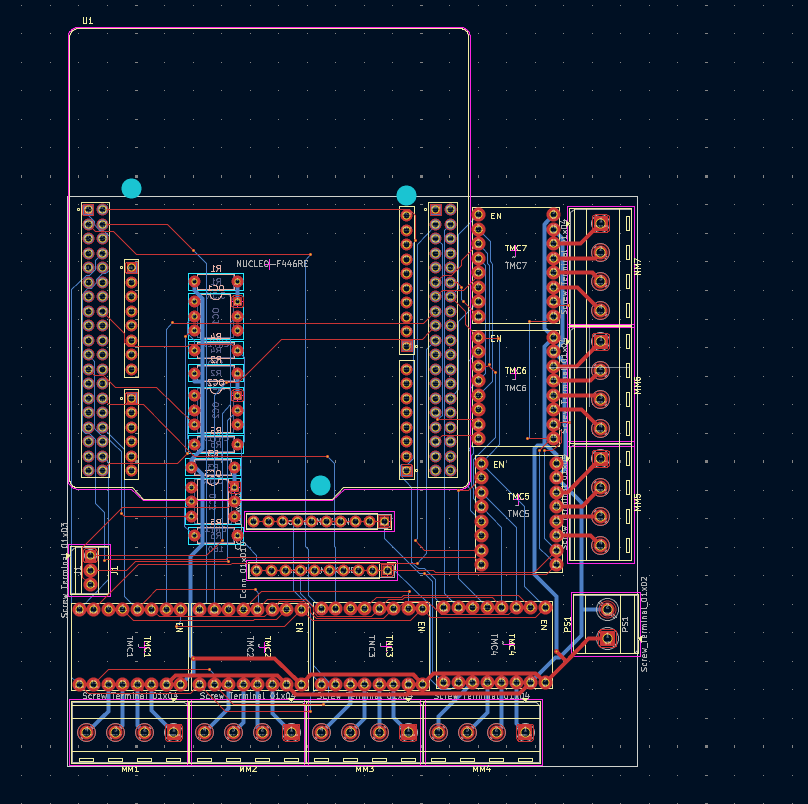
\includegraphics[width=0.8\textwidth]{images/pcb.png}
    \caption{Control Board PCB Layout}
    \label{fig:control_board_pcb}
\end{figure}

% TODO: Add 3D render
\begin{figure}[H]
    \centering
    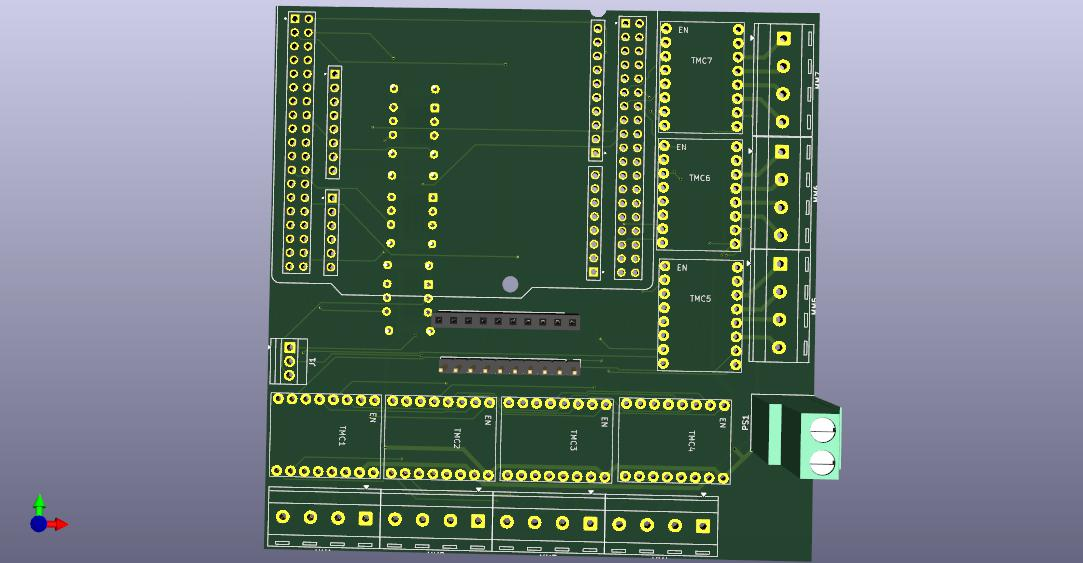
\includegraphics[width=0.8\textwidth]{images/3dpcb.jpg}
    \caption{Control Board 3D View}
    \label{fig:control_board_3d}
\end{figure}

\subsubsection{Key Features}

\begin{itemize}
    \item \textbf{MCU Interface}: Socket for STM32 Nucleo development board
    \item \textbf{Motor Drivers}: 7× TMC5160 BigTreeTech driver slots (6 robot joints + 1 gripper)
    \item \textbf{Motor Outputs}: Connectors for all stepper motors
    \item \textbf{Limit Switches}: Input connectors for all joint limit switches
    \item \textbf{Power Interface}: Motor power input and distribution
\end{itemize}

\subsection{Microcontroller}

The control board uses an \textbf{STM32 Nucleo} development board as the main processor:
\begin{itemize}
    \item Plugs into dedicated socket on the control board
    \item Provides all GPIO, timer, and communication interfaces
    \item USB connection for host communication
    \item Firmware development and debugging via ST-Link
\end{itemize}

\subsection{Motor Drivers}

The board accommodates 7 \textbf{TMC5160 BigTreeTech} stepper drivers:

\begin{table}[H]
    \centering
    \begin{tabular}{|c|l|l|}
        \hline
        \textbf{Slot} & \textbf{Function} & \textbf{Motor} \\
        \hline
        1 & Joint 1 & Base rotation \\
        2 & Joint 2 & Shoulder \\
        3 & Joint 3 & Elbow \\
        4 & Joint 4 & Wrist 1 \\
        5 & Joint 5 & Wrist 2 \\
        6 & Joint 6 & Wrist 3 \\
        7 & Gripper & End effector \\
        \hline
    \end{tabular}
    \caption{Motor Driver Assignments}
    \label{tab:driver_assignments}
\end{table}

\subsection{Power System}

\begin{itemize}
    \item \textbf{Motor Power}: Direct connection for motor supply voltage
    \item \textbf{Logic Power}: Regulated from motor supply or USB
\end{itemize}

\subsection{Connectors}

\begin{itemize}
    \item \textbf{Motor outputs}: 7× stepper motor connectors (4-pin)
    \item \textbf{Limit switches}: Input connectors for each joint
    \item \textbf{Encoder inputs}: For AS5600 position feedback
    \item \textbf{Power input}: Main power connector
\end{itemize}

%% --- Section 3: Electrical Connections ---
\section{Electrical Connections}

This section presents the schematic diagrams for the main electrical subsystems.

\subsection{MCU Connections}

The STM32 Nucleo board interfaces with all other subsystems:

\begin{figure}[H]
    \centering
    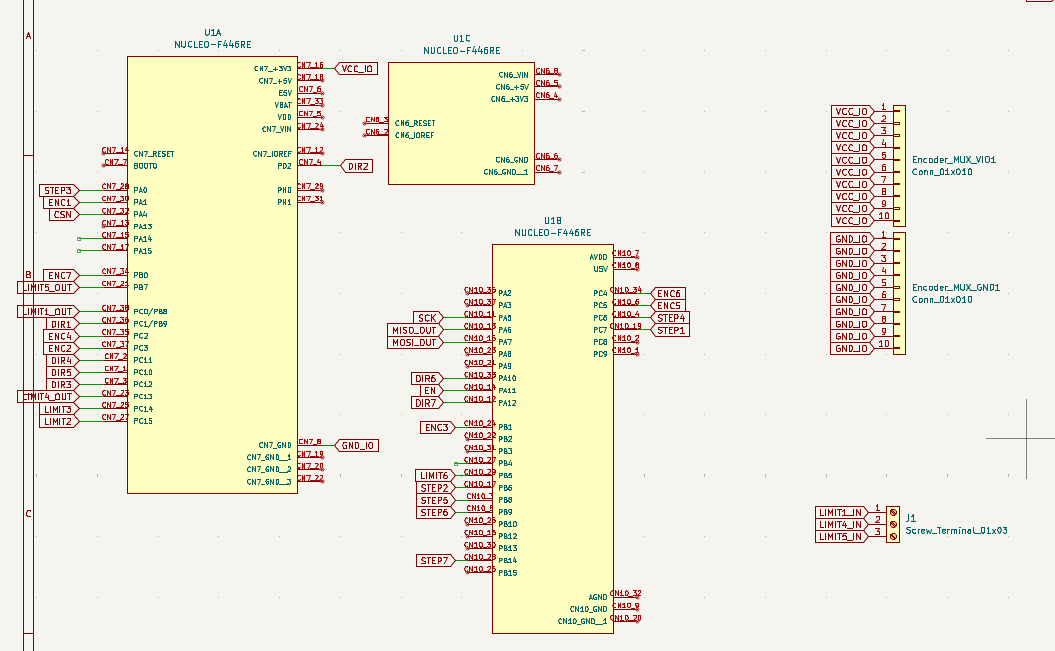
\includegraphics[width=0.9\textwidth]{images/mcu_schematics.png}
    \caption{MCU Schematic - STM32 Nucleo Connections}
    \label{fig:mcu_schematic}
\end{figure}

\subsection{Motor Driver Wiring}

The TMC5160 motor drivers are connected via \textbf{SPI daisy chain} configuration. This allows all 7 drivers to share a single SPI bus, reducing the number of required GPIO pins.

\begin{figure}[H]
    \centering
    
\includegraphics[width=0.9\textwidth]{"images/motor schematics.png"}
    \caption{Motor Driver Schematic - SPI Daisy Chain Configuration}
    \label{fig:motor_schematic}
\end{figure}

\subsubsection{SPI Daisy Chain}

In daisy chain mode:
\begin{itemize}
    \item All drivers share common SCK (clock) and CS (chip select) lines
    \item Data passes from SDO of one driver to SDI of the next
    \item Single SPI transaction addresses all 7 drivers sequentially
    \item Reduces wiring complexity and MCU pin usage
\end{itemize}

\subsection{Limit Switch Wiring}

Each joint has a limit switch for homing and end-of-travel protection:

\begin{figure}[H]
    \centering
    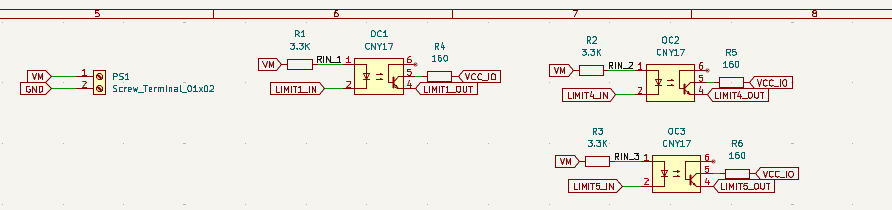
\includegraphics[width=0.7\textwidth]{images/limit_switch_sch.png}
    \caption{Limit Switch Schematic}
    \label{fig:limit_switch_schematic}
\end{figure}

%% ========================================
%% PART 3: MCU FIRMWARE
%% ========================================

\chapter{MCU Firmware}

This chapter describes the firmware running on the STM32 Nucleo microcontroller.

\section{Firmware Overview}

The MCU firmware is responsible for real-time motor control, sensor reading, and communication with the host. It uses FreeRTOS for task management.

\subsection{System Architecture}

\begin{figure}[H]
    \centering
    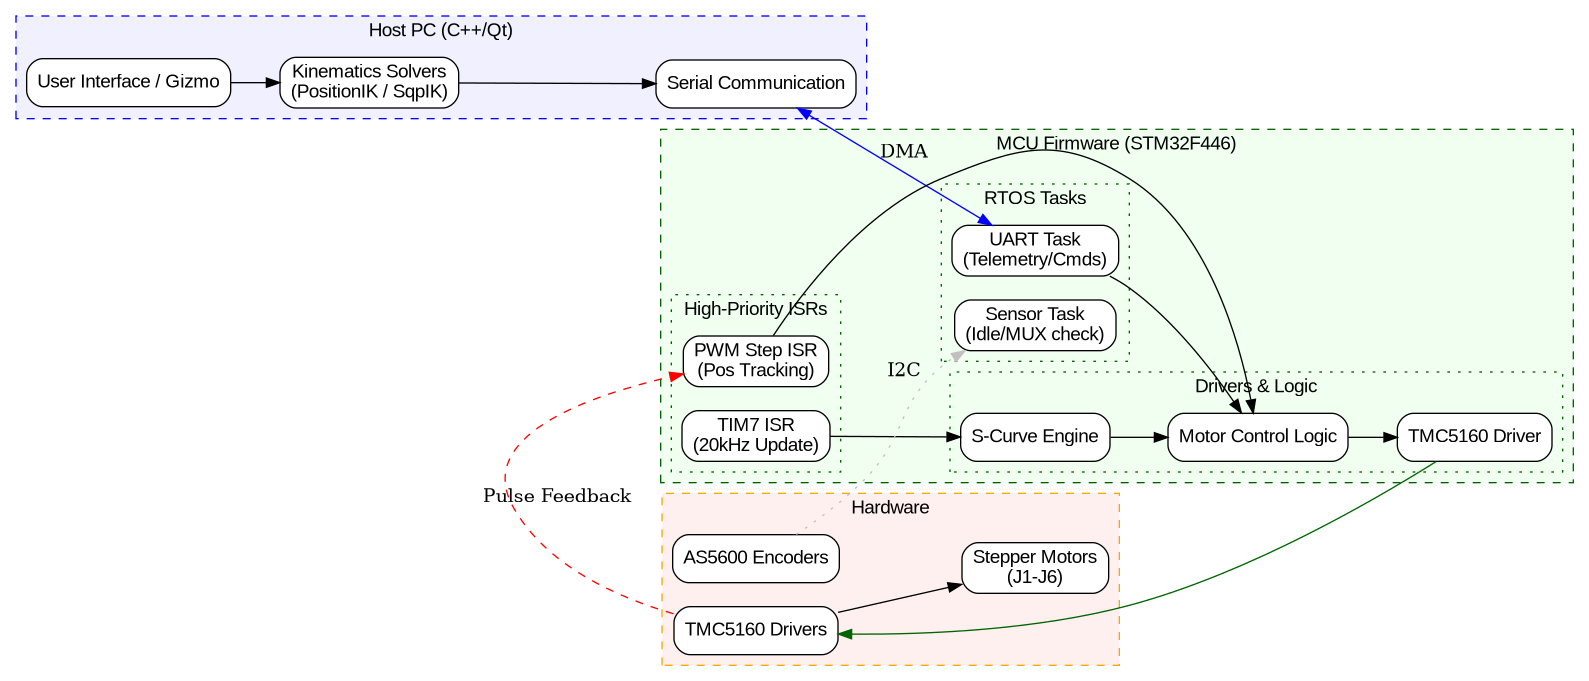
\includegraphics[width=1.0\textwidth]{images/system_architecture.png}
    \caption{System Architecture and Data Flow across Host PC, MCU, and Hardware}
    \label{fig:system_architecture}
\end{figure}

\subsection{RTOS Tasks}

The firmware utilizes a hybrid architecture combining high-frequency interrupts for motion control with RTOS tasks for communication and low-priority monitoring:

\begin{table}[H]
    \centering
    \begin{tabular}{|l|l|l|}
        \hline
        \textbf{Component} & \textbf{Priority/Rate} & \textbf{Function} \\
        \hline
        TIM7 ISR & 20\,kHz & S-Curve engine update, PWM frequency modulation \\
        PWM Step ISR & Event-based & Real-time position tracking, target-reached stopping \\
        UART Task & High & DMA-based telemetry streaming and command parsing \\
        Sensor Task & Low & PCA9548A MUX detection and health monitoring \\
        \hline
    \end{tabular}
    \caption{Real-Time Software Components}
    \label{tab:realtime_components}
\end{table}

\section{Motor Control}

\subsection{TMC5160 Driver Interface}

The firmware communicates with TMC5160 drivers via SPI:
\begin{itemize}
    \item Daisy chain configuration for all 7 drivers
    \item Register access for current, velocity, and position control
    \item StallGuard feedback for sensorless homing
\end{itemize}

\subsection{Step Generation}

Motor steps are generated using hardware timers:
\begin{itemize}
    \item Timer-based step pulse generation
    \item Velocity and acceleration limiting
    \item Smooth start/stop transitions
\end{itemize}

The firmware implements a high-performance 7-segment S-Curve motion profile to ensure continuous acceleration and minimize mechanical vibrations. Unlike standard trapezoidal profiles, the S-Curve limits the third derivative of position (jerk), preventing the "infinite jerk" spikes that lead to motor skipping and structural resonance.

\subsection{Mathematical Foundation}

The motion profile is governed by the constant jerk $J$, which is the rate of change of acceleration $a$. The kinematic states are derived through successive integration:

\begin{equation}
    a(t) = a_0 + \int_{0}^{t} J(\tau) d\tau
\end{equation}
\begin{equation}
    v(t) = v_0 + \int_{0}^{t} a(\tau) d\tau = v_0 + a_0 t + \frac{1}{2} J t^2
\end{equation}
\begin{equation}
    s(t) = s_0 + \int_{0}^{t} v(\tau) d\tau = s_0 + v_0 t + \frac{1}{2} a_0 t^2 + \frac{1}{6} J t^3
\end{equation}

\subsection{The 7-Segment Profile}

A full point-to-point motion consists of seven distinct phases:

\begin{enumerate}
    \item \textbf{Jerk-up}: Jerk is constant ($+J_{max}$), acceleration increases linearly.
    \item \textbf{Constant Accel}: Jerk is zero, acceleration is constant ($a_{max}$).
    \item \textbf{Jerk-down}: Jerk is constant ($-J_{max}$), acceleration decreases to zero as velocity reaches the maximum setpoint.
    \item \textbf{Constant Velocity}: Jerk and acceleration are zero.
    \item \textbf{Jerk-down}: Jerk is constant ($-J_{max}$), acceleration linearly decreases (deceleration increases).
    \item \textbf{Constant Decel}: Jerk is zero, deceleration is constant ($-a_{max}$).
    \item \textbf{Jerk-up}: Jerk is constant ($+J_{max}$), deceleration returns to zero as the target position is reached.
\end{enumerate}

\subsection{Implementation Strategy}

The firmware executes this engine within the \textbf{TIM7 ISR at 20\,kHz}. This high frequency (50\,$\mu$s ticks) allows for quasi-continuous updates of the output PWM frequency, ensuring the motor follows the ideal curve with negligible quantization error.

\subsubsection{Adaptive Deceleration}
Because the MCU must handle dynamic target updates and external interruptions, the engine does not simply "blindly" run a pre-calculated curve. Instead, it performs a \textbf{deceleration check every 1\,ms}:
\begin{itemize}
    \item It continuously calculates the \textit{stopping distance} required to reach zero velocity from the current speed using maximum jerk/decel limits.
    \item When the \textit{remaining distance} to the target is less than or equal to the stopping distance, it triggers the transition from constant velocity to the deceleration phases (Phase 5).
    \item \textbf{Overshoot Correction}: In the final pulses (Phase 7), any remaining floating-point error is compensated by an adaptive "dist-remove-per-cycle" calculation, guaranteeing that the final pulse lands exactly on the integer step target.
\end{itemize}

\section{Communication Protocol}

Communication with the host software is implemented over a high-speed USB-CDC serial link (baud rate 921,600). The protocol uses a robust binary framing to ensure data integrity and low latency.

\subsection{Framing Structure}
All packets, regardless of direction, share a common header and footer structure:
\begin{itemize}
    \item \textbf{Start Frame}: \texttt{0xAA 0x55} (2 bytes)
    \item \textbf{Length}: Payload size (2 bytes, Little-Endian)
    \item \textbf{Payload}: Actual data (variable length)
    \item \textbf{Checksum}: XOR sum of all payload bytes (1 byte)
\end{itemize}

\subsection{Outgoing Format (MCU $\rightarrow$ PC)}
The MCU streams telemetry at 100\,Hz. The primary telemetry packet (Type \texttt{0x01}) payload consists of:
\begin{itemize}
    \item \textbf{Joint Data}: 6 joints $\times$ (Position, Velocity, Acceleration) as 32-bit floats (72 bytes total)
    \item \textbf{Robot State}: 1 byte integer (Current operational mode)
\end{itemize}

\subsection{Incoming Format (PC $\rightarrow$ MCU)}
The host sends control and motion commands. The payload structure varies by command type:
\begin{itemize}
    \item \textbf{State Commands}: 1 byte (e.g., CMD\_ESTOP, CMD\_HOME)
    \item \textbf{Motion Commands}: 2 bytes (Command Type + Action) followed by 6 joints $\times$ (Position, Velocity) as 32-bit floats (50 bytes total)
\end{itemize}

%% ========================================
%% PART 4: URDF STANDALONE & MOTION CONTROL
%% ========================================

\chapter{Motion Control Software and Kinematics}

This chapter describes the kinematics theory and the host-side software for computation and control.

\section{Kinematics Theory}

Kinematics describes the motion of the robot without considering the forces that cause it. For our 6-DOF arm, we define the relationship between joint space $\mathbf{q} \in \mathbb{R}^6$ and task space $\mathbf{x} \in SE(3)$.

\subsection{Forward Kinematics}

Forward Kinematics (FK) is the mathematical process of determining the pose (position and orientation) of the end-effector given a set of joint angles. For a 6-DOF manipulator like our arm, this involves mapping a vector of joint angles $\mathbf{q} = [q_1, q_2, q_3, q_4, q_5, q_6]^T$ to a homogeneous transformation matrix ${}^0T_6 \in SE(3)$.

\begin{figure}[H]
    \centering
    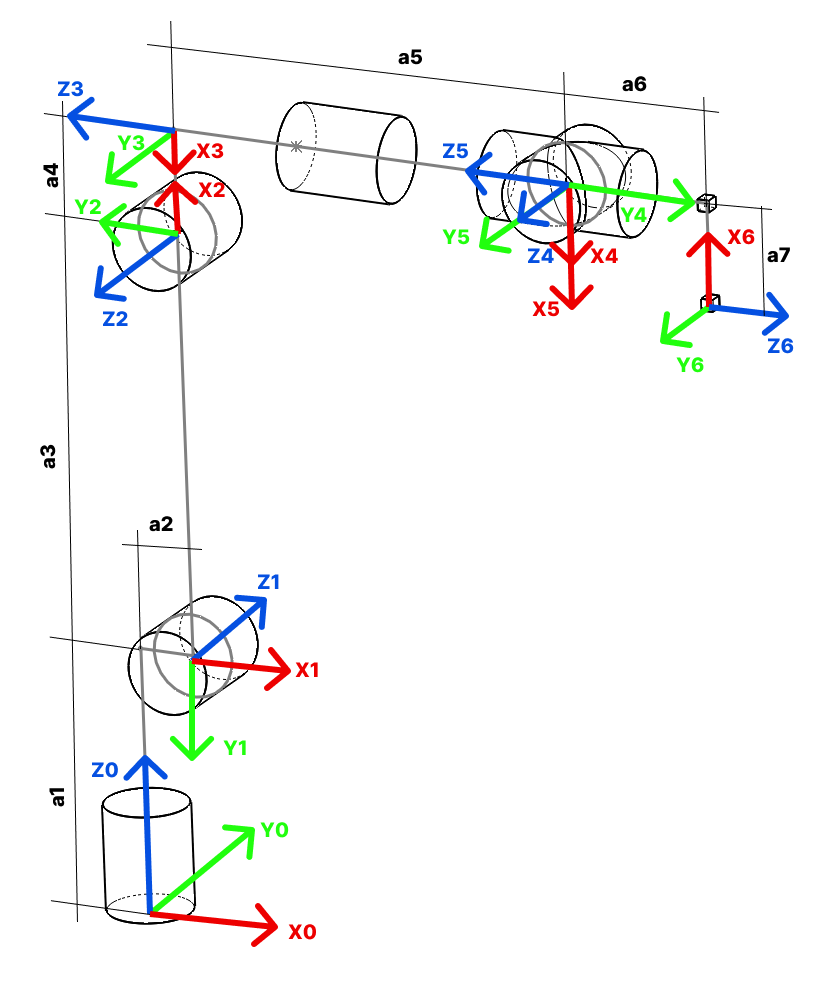
\includegraphics[width=0.8\textwidth]{images/robot_kinematic_diagram.png}
    \caption{Robot Kinematic Diagram showing joint axes and coordinate frames}
    \label{fig:kinematic_diagram}
\end{figure}

\subsubsection{The Denavit-Hartenberg (DH) Convention}

To systematically represent the relationship between adjacent links, we adopt the \textbf{Standard Denavit-Hartenberg (DH)} convention. This method assigns a coordinate frame to each joint and describes the transformation from frame $i-1$ to frame $i$ using four parameters:

\begin{itemize}
    \item \textbf{Joint Angle} ($\theta_i$): Rotation about the $z_{i-1}$ axis. This is the variable component for revolute joints.
    \item \textbf{Link Offset} ($d_i$): Distance along the $z_{i-1}$ axis from the origin of frame $i-1$ to the common normal between $z_{i-1}$ and $z_i$.
    \item \textbf{Link Length} ($a_i$): Distance along the $x_i$ axis (the common normal) between the $z_{i-1}$ and $z_i$ axes.
    \item \textbf{Link Twist} ($\alpha_i$): Rotation about the $x_i$ axis required to align $z_{i-1}$ with $z_i$.
\end{itemize}

The individual transformation matrix ${}^{i-1}T_i$ is the result of four successive operations: $Rot_z(\theta_i) \to Trans_z(d_i) \to Trans_x(a_i) \to Rot_x(\alpha_i)$.

\begin{equation}
    {}^{i-1}T_i = 
    \begin{bmatrix}
    \cos\theta_i & -\sin\theta_i\cos\alpha_i & \sin\theta_i\sin\alpha_i & a_i\cos\theta_i \\
    \sin\theta_i & \cos\theta_i\cos\alpha_i & -\cos\theta_i\sin\alpha_i & a_i\sin\theta_i \\
    0 & \sin\alpha_i & \cos\alpha_i & d_i \\
    0 & 0 & 0 & 1
    \end{bmatrix}
\end{equation}

\subsubsection{Robot DH Parameters}

Based on the physical dimensions of our robot arm, the following DH parameters define the kinematic chain. The base height $H_1$, link lengths $L_2, L_3$, and wrist offsets $W_1, W_2$ are derived from the URDF model.

\begin{figure}[H]
    \centering
    \begin{minipage}{0.48\textwidth}
        \centering
        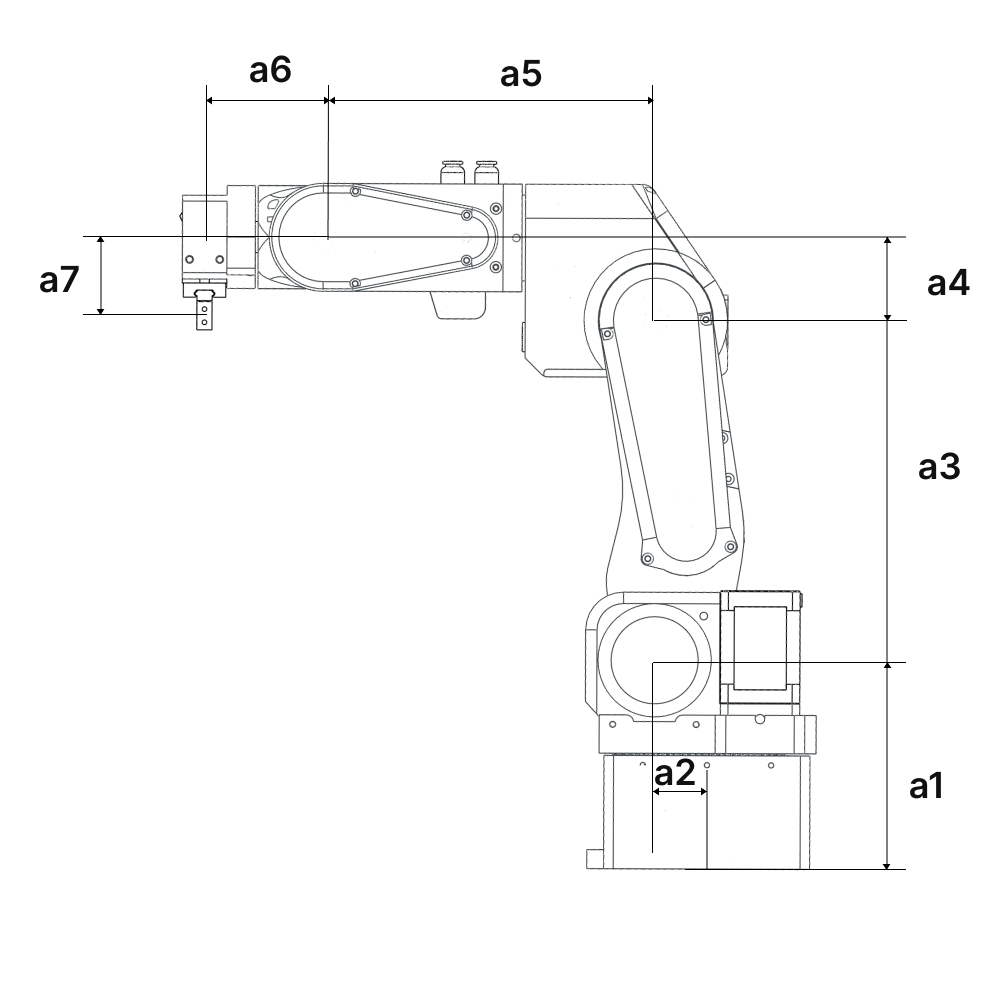
\includegraphics[width=\textwidth]{images/robot_link_lengths.png}
        \caption{Physical Link Lengths}
        \label{fig:link_lengths}
    \end{minipage}
    \hfill
    \begin{minipage}{0.48\textwidth}
        \centering
        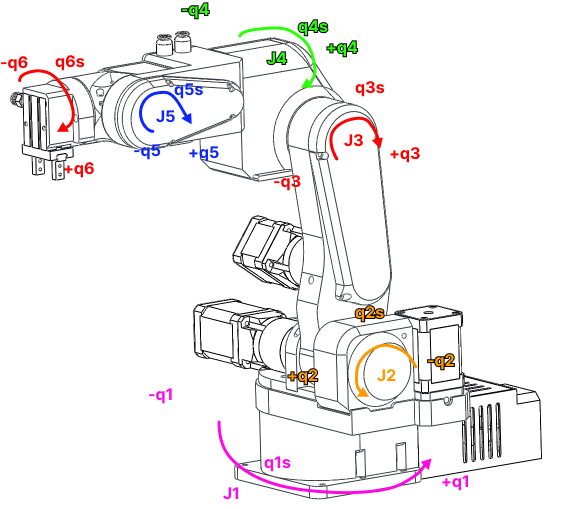
\includegraphics[width=\textwidth]{images/robot_rotation.png}
        \caption{Joint Rotation Directions}
        \label{fig:robot_rotation}
    \end{minipage}
\end{figure}

\begin{table}[H]
    \centering
    \begin{tabular}{|c|c|c|c|c|}
        \hline
        \textbf{Link} & $\theta_i$ & $d_i$ & $a_i$ & $\alpha_i$ \\
        \hline
        1 & $q_1$ & $110.5\,$mm & $23.4\,$mm & $-90^\circ$ \\
        2 & $q_2$ & $0\,$mm & $180.0\,$mm & $180^\circ$ \\
        3 & $q_3$ & $0\,$mm & $43.5\,$mm & $90^\circ$ \\
        4 & $q_4$ & $176.35\,$mm & $0\,$mm & $-90^\circ$ \\
        5 & $q_5$ & $0\,$mm & $51.0\,$mm & $90^\circ$ \\
        6 & $q_6$ & $52.0\,$mm & $0\,$mm & $0^\circ$ \\
        \hline
    \end{tabular}
    \caption{DH Parameters for the 6-DOF Robot Arm}
    \label{tab:dh_parameters}
\end{table}

The total transformation from the base to the end-effector is obtained by multiplying these matrices in sequence:
\begin{equation}
    {}^{0}T_{ee}(\mathbf{q}) = {}^{0}T_1(q_1) \cdot {}^{1}T_2(q_2) \cdot {}^{2}T_3(q_3) \cdot {}^{3}T_4(q_4) \cdot {}^{4}T_5(q_5) \cdot {}^{5}T_6(q_6)
\end{equation}

\subsubsection{End-Effector Pose Extraction}

The resulting $4 \times 4$ homogeneous transformation matrix ${}^0T_{ee}$ contains the full pose information relative to the base frame. It is partitioned as follows:

\begin{equation}
    {}^0T_{ee} = \begin{bmatrix}
    \mathbf{n} & \mathbf{s} & \mathbf{a} & \mathbf{p} \\
    0 & 0 & 0 & 1
    \end{bmatrix} = \begin{bmatrix}
    r_{11} & r_{12} & r_{13} & p_x \\
    r_{21} & r_{22} & r_{23} & p_y \\
    r_{31} & r_{32} & r_{33} & p_z \\
    0 & 0 & 0 & 1
    \end{bmatrix}
\end{equation}

where:
\begin{itemize}
    \item \textbf{Position}: The vector $\mathbf{p} = [p_x, p_y, p_z]^T$ represents the Cartesian coordinates of the end-effector origin.
    \item \textbf{Orientation}: The $3 \times 3$ submatrix $\mathbf{R} = [\mathbf{n}, \mathbf{s}, \mathbf{a}]$ represents the rotation of the end-effector. The columns $\mathbf{n}$ (normal), $\mathbf{s}$ (sliding), and $\mathbf{a}$ (approach) are unit vectors defining the orientation of the final link's axes in the base frame.
\end{itemize}

In our software, this position vector and rotation matrix are used directly for error computation in the numerical solvers and for visualization in the 3D interface.

\subsection{The Jacobian Matrix}

The Jacobian matrix $\mathbf{J}(\mathbf{q})$ is a fundamental operator in robotics that maps velocities from joint space to task space. For our 6-DOF manipulator, it relates the joint velocity vector $\dot{\mathbf{q}} \in \mathbb{R}^6$ to the end-effector twist $\mathbf{\xi} = [\mathbf{v}, \mathbf{\omega}]^T \in \mathbb{R}^6$:

\begin{equation}
    \begin{bmatrix} \mathbf{v} \\ \mathbf{\omega} \end{bmatrix} = \mathbf{J}(\mathbf{q}) \dot{\mathbf{q}}
\end{equation}

where $\mathbf{v}$ is the linear velocity and $\mathbf{\omega}$ is the angular velocity of the end-effector.

\subsubsection{Geometric Jacobian Derivation}

The Jacobian is composed of six columns, $\mathbf{J} = [\mathbf{j}_1, \mathbf{j}_2, \dots, \mathbf{j}_6]$, where each column represents the contribution of a single joint to the end-effector velocity. Since all joints in our robot are revolute, the $i$-th column is derived geometrically as:

\begin{equation}
    \mathbf{j}_i = \begin{bmatrix} \mathbf{z}_{i-1} \times (\mathbf{p}_{ee} - \mathbf{p}_{i-1}) \\ \mathbf{z}_{i-1} \end{bmatrix}
\end{equation}

where:
\begin{itemize}
    \item $\mathbf{z}_{i-1}$ is the unit vector along the axis of rotation of joint $i$.
    \item $\mathbf{p}_{ee}$ is the position of the end-effector in the base frame.
    \item $\mathbf{p}_{i-1}$ is the position of the origin of frame $i-1$ in the base frame.
\end{itemize}

The Jacobian is highly configuration-dependent. When $\mathbf{J}(\mathbf{q})$ becomes singular (loses rank), the robot loses one or more degrees of freedom in task space. This occurs when joint axes align or the arm reaches its workspace boundaries.

\subsection{Singularity Handling: Selectively Damped Least Squares}

To maintain stability near singularities, we utilize the \textbf{Selectively Damped Least Squares (SDLS)} method. Unlike standard Damped Least Squares (Tikhonov regularization) which adds a uniform penalty to all joints, SDLS specifically targets only the singular directions in the task space.

Through Singular Value Decomposition (SVD), the Jacobian is decomposed as:
\begin{equation}
    \mathbf{J} = \mathbf{U} \mathbf{\Sigma} \mathbf{V}^T
\end{equation}
where the columns of $\mathbf{V}$ are joint-space vectors. We construct a damping matrix $\mathbf{\Lambda}$ that acts only in the basis of these vectors:
\begin{equation}
    \mathbf{\Lambda} = \sum_{i=1}^{n} \lambda_i^2 \mathbf{v}_i \mathbf{v}_i^T
\end{equation}
The per-mode damping factor $\lambda_i$ is computed based on the singular value $\sigma_i$:
\begin{equation}
    \lambda_i = \begin{cases} 
    \lambda_{max} \left(1 - \frac{\sigma_i}{\sigma_{threshold}}\right)^2 & \text{if } \sigma_i < \sigma_{threshold} \\
    0 & \text{otherwise}
    \end{cases}
\end{equation}
This approach ensures that "healthy" directions remain precise while "singular" directions are smoothly constrained, preventing infinite joint speeds and numerical instability.

\subsection{Inverse Kinematics}

Inverse Kinematics (IK) is the process of finding the joint angles $\mathbf{q}$ that result in a desired end-effector pose. Unlike FK, IK is non-linear and can have multiple solutions, or no solution if the target is outside the workspace.

\subsubsection{Analytical Inverse Kinematics}

Analytical (closed-form) Inverse Kinematics is the process of finding joint angles $\mathbf{q}$ algebraically. Our robot's architecture allows for a \textbf{kinematic decoupling} strategy, which divides the 6-DOF problem into two smaller, independent subproblems: a 3-DOF positional problem and a 3-DOF orientational problem.

\paragraph{1. Kinematic Decoupling (Wrist Center)}

The key requirement for decoupling is that the axes of the last three joints (Joints 4, 5, and 6) intersect at a single point, known as the \textbf{wrist center} ($P_w$). Because rotational motion of the wrist does not move $P_w$, its position is determined solely by the first three joints.

Given a target end-effector position $\mathbf{p}_{target}$ and its approach vector $\mathbf{a}$ (the $z$-axis of the end-effector frame), the wrist center is calculated as:
\begin{equation}
    \mathbf{p}_w = \mathbf{p}_{target} - d_6 \cdot \mathbf{a}
\end{equation}
where $d_6 = 52.0\,$mm is the distance from the wrist center to the end-effector tip.

\paragraph{2. Solving for the Arm (Joints 1, 2, 3)}

With $\mathbf{p}_w = [x_w, y_w, z_w]^T$ known in the base coordinate frame:
\begin{itemize}
    \item \textbf{Base Rotation ($q_1$)}: The first joint rotates the entire arm to align with the $x-y$ projection of the wrist center:
    \begin{equation}
        q_1 = \operatorname{atan2}(y_w, x_w) \quad (\text{or } q_1 + \pi \text{ for reversed base})
    \end{equation}
    \item \textbf{Planar Geometry ($q_2, q_3$)}: Once $q_1$ is fixed, the problem simplifies to a 2D planar linkage. We solve for $q_2$ and $q_3$ using the \textbf{Law of Cosines} based on the triangle formed by $L_2$, $L_3$, and the radial distance to $P_w$. This step yields two solutions per base configuration: \textit{Elbow Up} and \textit{Elbow Down}.
\end{itemize}

\paragraph{3. Solving for the Wrist (Joints 4, 5, 6)}

After calculating the arm joints, the rotation matrix from the base to Joint 3, ${}^{0}R_3$, is fully defined. To reach the target orientation $\mathbf{R}_{target}$, the wrist must provide the remaining rotation ${}^{3}R_6$:
\begin{equation}
    {}^{3}R_6 = ({}^{0}R_3)^T \cdot \mathbf{R}_{target}
\end{equation}
The matrix ${}^{3}R_6$ corresponds to a standard \textbf{Z-Y-Z Euler sequence} defined by the wrist joints $q_4, q_5, q_6$. Equating the elements of ${}^{3}R_6$ to the Euler rotation matrix allows us to extract the angles:
\begin{equation}
    q_5 = \pm \operatorname{acos}(R_{33}) \quad (\text{where } R_{33} \text{ is the bottom-right element})
\end{equation}
The choice of sign for $q_5$ defines the \textbf{Wrist Flip} (normalized vs. flipped configuration).

\paragraph{4. Solution Selection and Configuration Ranking}

For any reachable target, the analytical solver \cite{EAIK} generates a candidate set of up to \textbf{8 valid solutions} (2 Base $\times$ 2 Elbow $\times$ 2 Wrist). Because analytical IK can be discontinuous—exhibiting "jerk" between branches—our solver utilizes a ranking and blending system to select the most stable solution:

\begin{itemize}
    \item \textbf{Configuration Hysteresis}: A large "Branch Penalty" is applied to solutions that require a change in the robot's fundamental mode (e.g., flipping the base or elbow). This ensures the robot stays within its current kinematic branch as long as it is reachable.
    \item \textbf{Singularity-Aware Metric}: Standard Euclidean distance is insufficient near singularities. Our metric downweights Joint 4 and 6 when near a wrist singularity ($|\sin(q_5)| \approx 0$), as they become redundant. We also penalize deviations in the joint sum $q_4 + q_6$ to maintain consistent orientation.
    \item \textbf{Dynamic Blend Zones}: We implement a \textit{Lock-and-Blend} strategy. Below a $3^\circ$ threshold, Joint 4 and 6 are hard-locked to their previous values. Between $3^\circ$ and $8^\circ$, a linear blend factor smoothly transitions the solution from the previous state to the new analytical goal.
    \item \textbf{Manipulability Ranking}: Solutions are ranked using the \textit{Yoshikawa Manipulability Index} ($\sqrt{\det(J J^T)}$) \cite{mathworks}. Configurations that are further away from geometric singularities (vertical arm, fully extended elbow) are prioritized.
    \item \textbf{Velocity-Aware Penalty}: The solver predicts the required joint velocity ($\dot{q} = \Delta q / \Delta t$). Solutions that would require velocities exceeding the motor's physical limits are heavily penalized to avoid physical tripping.
\end{itemize}

\subsection{Role in the Control Loop}

It is important to note that this \textbf{Analytical Inverse Kinematics} solver \cite{EAIK} is primarily used for \textbf{simulation and global initialization}. Because it is solved algebraically at a discrete pose, it is not inherently continuous. In the real-time control system, it serves as a \textbf{Seeder} for the \textbf{Differential QP Controller} (described in Section 4.3). The analytical solver provides a globally valid starting point, while the QP-based Jacobian solver ensures perfectly smooth, continuous joint trajectories during execution.




\section{Differential IK via Quadratic Programming: A Constraint-Aware Framework}

\subsection*{Executive Summary}
This report details our \textbf{Differential QP Controller}, which hybridizes analytical seeding with a numerical Quadratic Programming (QP) solver. By integrating \textbf{Selectively Damped Least Squares (SDLS)} and strict physical constraints via OSQP, the controller ensures robust, singularity-aware motion that overcomes the limitations of traditional numerical methods.

\subsection{Introduction and Problem Formulation}

\subsubsection{The Kinematic Control Challenge in Modern Robotics}
Inverse Kinematics (IK) constitutes the foundational layer of robotic manipulation, serving as the critical mathematical bridge between high-level task planning in Cartesian space and the low-level joint servo control required by actuators. The problem is formally defined as finding a joint configuration vector $\mathbf{q} \in \mathbb{R}^n$ that satisfies the non-linear mapping $\mathbf{x}_{des} = f(\mathbf{q})$, where $\mathbf{x}_{des} \in SE(3)$ represents the desired end-effector pose and $f: \mathbb{R}^n \rightarrow SE(3)$ is the forward kinematics function.

While this formulation appears straightforward, practical implementation in industrial and collaborative environments introduces significant complexity. The function $f(\mathbf{q})$ is highly non-linear, involving trigonometric compositions that result in non-convex solution spaces. Redundant manipulators possess an infinite set of solutions known as the self-motion manifold. Conversely, non-redundant manipulators may have multiple discrete geometric solutions (branches), such as "elbow-up" or "elbow-down" configurations.

\subsubsection{Limitations of Classical Numerical Solvers}
Historically, the robotics community has relied on analytical and numerical solvers. Analytical solvers are fast and complete but specific to geometry and cannot easily incorporate inequality constraints. Numerical iterative methods offer generality by solving the problem at the velocity level:
\begin{equation}
    \dot{\mathbf{x}} = \mathbf{J}(\mathbf{q})\dot{\mathbf{q}}
\end{equation}
where $\mathbf{J}(\mathbf{q}) = \partial f / \partial \mathbf{q} \in \mathbb{R}^{m \times n}$ is the manipulator Jacobian. However, these classical numerical approaches suffer from three critical pathologies:
\begin{itemize}
    \item \textbf{Local Minima Entrapment}: Gradient-based solvers descend the error landscape from an initial guess. If initialized in the basin of attraction of a local minimum, the solver may converge to a state where the Cartesian error is non-zero, yet no local movement can reduce it.
    \item \textbf{Singularity Instability}: Near kinematic singularities (where $\text{rank}(\mathbf{J}) < m$), the Jacobian becomes ill-conditioned. Pseudoinverse-based controllers command infinite joint velocities, leading to dangerous "jerk" or controller divergence.
    \item \textbf{Constraint Violation}: Pure kinematic inversion ($\dot{\mathbf{q}} = \mathbf{J}^\dagger \dot{\mathbf{x}}$) is fundamentally unconstrained. It does not natively ensure that the resulting joint coordinates $\mathbf{q}$ remain within physical limits.
\end{itemize}

\subsubsection{The Optimization Paradigm: Differential QP}
Our controller addresses these limitations by reformulating the IK problem as a \textbf{Constrained Quadratic Program (QP)}. By expressing the control objective as the minimization of a quadratic cost function subject to linear inequality constraints, the controller can optimally trade off tracking error against control effort while rigorously respecting physical boundaries. 

This implementation utilizes the \textbf{OSQP (Operator Splitting Quadratic Program)} solver, a numerical engine tailored for sparse, convex problems. Crucially, the controller augments this optimization core with a \textbf{Hybrid Architecture}, utilizing an analytical solver \cite{EAIK} to seed the optimization. This combines the global topology awareness of analytical methods with the local constraint-handling capability of numerical optimization.

\subsection{Mathematical Framework and Derivations}
The efficacy of the controller rests on a rigorous mathematical formulation that translates physical robotic constraints into the language of convex optimization.

\subsubsection{Differential Kinematics and Error Dynamics}
The controller operates in a closed-loop real-time cycle (1 kHz). At each timestep $t$, the goal is to compute a joint velocity vector $\dot{\mathbf{q}}$ that minimizes the error between the current pose and the target pose.

\paragraph{Task-Space Error Formulation}
The translational error $\mathbf{e}_p$ is the linear difference: $\mathbf{e}_p = \mathbf{p}_{target} - \mathbf{p}_{current}$. The rotational error $\mathbf{e}_o$ utilizes unit quaternions $\mathbf{Q} = [w, x, y, z]^T$. To handle the double cover of $SO(3)$, we explicitly check the inner product:
\begin{equation}
    \text{if } (\mathbf{Q}_{curr} \cdot \mathbf{Q}_{target} < 0) \implies \mathbf{Q}_{target} \leftarrow -\mathbf{Q}_{target}
\end{equation}
The orientation error is computed as: $\mathbf{e}_o = 2 \ln(\mathbf{Q}_{target} \otimes \mathbf{Q}_{curr}^{-1})$. This prevents "unwinding" jumps and ensures rotation along the geodesic path.

\paragraph{Reference Velocity Generation}
The controller employs a Proportional (P) control law in task space:
\begin{equation}
    \mathbf{v}_{ref} = K_p \begin{bmatrix} \mathbf{e}_p \\ \mathbf{e}_o \end{bmatrix}
\end{equation}
This linearizes the tracking dynamics, treating the robot as a first-order kinematic system.

\subsection{Differential QP-Based Inverse Kinematics (OSQP Formulation)}

\subsubsection{1. Optimization problem being solved}
At every control cycle, the solver computes a joint velocity command $\dot{\mathbf{q}} \in \mathbb{R}^n$ that best tracks a desired Cartesian velocity while respecting joint limits. The problem is formulated as the following convex quadratic program:
\begin{align}
    \min_{\dot{\mathbf{q}}} \quad & \frac{1}{2} || \mathbf{J}(\mathbf{q})\dot{\mathbf{q}} - \mathbf{v}_{ref} ||_{\mathbf{W}}^2 + \frac{1}{2} \dot{\mathbf{q}}^T \mathbf{\Lambda} \dot{\mathbf{q}} \\
    \text{s.t.} \quad & \dot{\mathbf{q}}_{min} \leq \dot{\mathbf{q}} \leq \dot{\mathbf{q}}_{max}
\end{align}
Where:
\begin{itemize}
    \item $\mathbf{J} \in \mathbb{R}^{6 \times n}$ is the geometric Jacobian.
    \item $\mathbf{v}_{ref} = K_p \mathbf{e}$ is the desired Cartesian velocity.
    \item $\mathbf{W}$ is a task-space weighting matrix.
    \item $\mathbf{\Lambda}$ is an adaptive SDLS damping matrix.
    \item Constraints enforce joint velocity and joint-limit damping bounds.
\end{itemize}

\subsubsection{2. Mapping to standard QP form (OSQP)}
OSQP solves problems of the form:
\begin{align}
    \min_{x} \quad & \frac{1}{2} x^T P x + q^T x \\
    \text{s.t.} \quad & l \leq A x \leq u
\end{align}
where $x \in \mathbf{R}^n$ is the optimization variable and $P \in \mathbf{S}^n_+$ a positive semidefinite matrix \cite{osqp}.

\subsubsection{3. Objective function mapping}
\paragraph{3.1 Quadratic term (Hessian)}
Expanding the least-squares objective:
\begin{equation}
    || \mathbf{J}\dot{\mathbf{q}} - \mathbf{v}_{ref} ||_{\mathbf{W}}^2 = \dot{\mathbf{q}}^T \mathbf{J}^T \mathbf{W} \mathbf{J} \dot{\mathbf{q}} - 2 \mathbf{v}_{ref}^T \mathbf{W} \mathbf{J} \dot{\mathbf{q}} + \text{const}
\end{equation}
Thus, the Hessian is defined as: $\mathbf{P} = \mathbf{J}^T \mathbf{W} \mathbf{J} + \mathbf{\Lambda}$. In practice, a small $\epsilon\mathbf{I}$ is added for numerical positive definiteness.
\begin{itemize}
    \item \textbf{Code mapping}:
\begin{lstlisting}[language=C++]
P_dense = J.transpose() * W_diag * J + Lambda;
P_dense += 1e-6 * Eigen::MatrixXd::Identity(num_joints_, num_joints_);
\end{lstlisting}
\end{itemize}

\paragraph{3.2 Linear term (gradient)}
The linear term of the QP is derived as: $\mathbf{q} = -\mathbf{J}^T \mathbf{W} \mathbf{v}_{ref}$.
\begin{itemize}
    \item \textbf{Code mapping}:
\begin{lstlisting}[language=C++]
q_grad_ = -J.transpose() * W_diag * v_ref;
\end{lstlisting}
\end{itemize}

\subsubsection{4. Constraints mapping}
\paragraph{4.1 Constraint matrix}
Only box constraints are enforced: $\dot{\mathbf{q}}_{min} \leq \dot{\mathbf{q}} \leq \dot{\mathbf{q}}_{max}$. This is implemented via an identity constraint matrix $\mathbf{A} = \mathbf{I}_{n \times n}$.
\begin{itemize}
    \item \textbf{Code mapping}:
\begin{lstlisting}[language=C++]
A_sparse_.setIdentity();
\end{lstlisting}
\end{itemize}

\paragraph{4.2 Velocity Dampers for Joint Constraints}
An implementation detail is the use of \textbf{Velocity Dampers} (also known as potential field limits or control barrier functions at the velocity level) to enforce position limits. This technique converts order-zero constraints (position) into order-one constraints (velocity), making them compatible with the differential QP formulation.

For a joint $i$ with position limits $[q_{min}^i, q_{max}^i]$ and physical velocity limits $[-v_{max}^i, v_{max}^i]$, the admissible velocity interval $[\dot{q}_{lower}^i, \dot{q}_{upper}^i]$ is dynamically adjusted based on the proximity to the limits.

The upper velocity bound is defined as:
\begin{equation}
    \dot{q}_{upper}^i(t) = \min \left( v_{max}^i, \quad \xi \frac{q_{max}^i - q_i(t)}{\Delta t} \right)
\end{equation}

The lower velocity bound is defined as:
\begin{equation}
    \dot{q}_{lower}^i(t) = \max \left( -v_{max}^i, \quad \xi \frac{q_{min}^i - q_i(t)}{\Delta t} \right)
\end{equation}
where $\xi$ is the \texttt{velocity\_damper\_gain\_} (typically $\xi \in [0.1, 1.0]$).

This formulation acts as a \textbf{"soft wall"}:
\begin{itemize}
    \item \textbf{Far from limit}: The term $\xi \frac{d_{limit}}{\Delta t}$ is large, so the bound is simply the physical motor limit $v_{max}$.
    \item \textbf{Approaching limit}: As the distance to the limit approaches zero, the allowable velocity linearly decreases, forcing the robot to decelerate smoothly.
    \item \textbf{At limit}: The velocity bound becomes zero (or negative), strictly preventing any motion that would violate the limit while permitting motion away from it.
\end{itemize}

These dynamic bounds are fed directly into the QP constraint vectors $l$ and $u$ ($l_{eff}$ and $u_{eff}$ in the code), ensuring that the optimization result is always \textbf{"viable"}---meaning a valid future trajectory exists.

\begin{table}[H]
\centering
\begin{tabular}{|l|l|l|}
\hline
\textbf{Constraint Type} & \textbf{Physical Meaning} & \textbf{Mathematical Implementation} \\ \hline
Box Constraint & Actuator Speed Limits & $\dot{q} \in [-v_{max}, v_{max}]$ \\ \hline
Barrier Constraint & Joint Position Limits & $\dot{q} \le \xi (q_{max} - q) / \Delta t$ \\ \hline
Optimization & Task Tracking & $\min || \mathbf{J}\dot{\mathbf{q}} - \mathbf{v}_{ref} ||^2$ \\ \hline
\end{tabular}
\end{table}

\begin{itemize}
    \item \textbf{Code mapping}:
\begin{lstlisting}[language=C++]
u_eff_(i) = vel_upper;
l_eff_(i) = -vel_lower;
\end{lstlisting}
\end{itemize}

\subsubsection{5. Selectively Damped Least Squares (SDLS)}
To avoid over-damping well-conditioned directions, damping is applied per singular mode \cite{buss}:
\begin{equation}
    \mathbf{\Lambda} = \sum_{i} \lambda_i^2 \mathbf{v}_i \mathbf{v}_i^T
\end{equation}
Where the per-mode damping $\lambda_i$ follows a quadratic ramp:
\begin{equation}
    \lambda_i = 
    \begin{cases} 
    \lambda_{max}(1 - \sigma_i / \sigma_{th})^2 & \text{if } \sigma_i < \sigma_{th} \\
    0 & \text{otherwise}
    \end{cases}
\end{equation}
\begin{itemize}
    \item \textbf{Code mapping}:
\begin{lstlisting}[language=C++]
Lambda += (lambda_i * lambda_i) * V.col(i) * V.col(i).transpose();
\end{lstlisting}
\end{itemize}
This preserves accuracy in non-singular directions while stabilizing the controller near rank-deficiencies.

\subsubsection{6. Final solved QP (summary)}
At each control step, OSQP solves the integrated objective:
\begin{align}
    \min_{\dot{\mathbf{q}}} \quad & \frac{1}{2} \dot{\mathbf{q}}^T (\mathbf{J}^T \mathbf{W} \mathbf{J} + \mathbf{\Lambda}) \dot{\mathbf{q}} - (\mathbf{J}^T \mathbf{W} \mathbf{v}_{ref})^T \dot{\mathbf{q}} \\
    \text{s.t.} \quad & \dot{\mathbf{q}}_{min} \leq \dot{\mathbf{q}} \leq \dot{\mathbf{q}}_{max}
\end{align}

\subsection{Hybrid Architecture: Topology and Global Awareness}
Behind the optimization core, the controller implements a Motion Lookahead and Hysteresis mechanism to navigate the robot's discrete configuration space.

\subsubsection{Predictive Motion Lookahead}
Instead of reacting only to the current error, the controller extrapolates the current trajectory to predict the robot's pose in the near future:
\begin{equation}
    \mathbf{p}_{lookahead} = \mathbf{p}_{current} + \frac{\mathbf{e}_{pos}}{||\mathbf{e}_{pos}||} \cdot \min(d_{lookahead}, ||\mathbf{e}_{pos}||)
\end{equation}
The analytical IK is solved for this future pose. This effectively asks: "If we continue moving in this direction, will we need to flip the elbow or wrist?" If the \texttt{detectBranch} function identifies that the future pose requires a different configuration branch, the controller prepares to switch. This "proto-MPC" behavior allows the robot to anticipate kinematic bifurcations rather than stumbling into them blindly.

\subsubsection{Hysteresis-Based Branch Switching}
To prevent "chattering"---the rapid, unstable oscillation between configuration branches when near a workspace boundary---the controller implements a hysteresis filter. A switch is only permitted if the cost benefit of switching exceeds a predefined threshold:
\begin{equation}
    \text{Cost}_{switch} < \text{Cost}_{stay} - \tau_{hysteresis}
\end{equation}
The cost function \texttt{computeBranchCost} penalizes joint distance and manipulability loss:
\begin{equation}
    \text{Cost}(q) = \sum (q_i - q_{current,i})^2 + \frac{1}{|\sin(q_{wrist})| + \epsilon}
\end{equation}
This logic ensures that the robot remains in its current valid configuration until the alternative becomes significantly better, mimicking the stability of biological motor control.

\subsection{Implementation and Performance Evaluation}
The system is implemented in C++ using the Eigen library and OSQP. We utilize \textbf{Warm-Starting} (initializing with the previous solution) to reduce solver iterations to $\sim 3-5$ per cycle, enabling $1\,$kHz performance.

We evaluate performance through:
\begin{itemize}
    \item \textbf{Singularity Transit}: Verifying stable velocity norms and graceful tracking degradation as $\sigma_{min} \to 0$.
    \item \textbf{Elbow Flip Testing}: Confirming 100\% reachability in configuration-switching scenarios where standard local solvers fail.
\end{itemize}


\section{Visualization and Control Interface}

The robot is operated via a custom graphical user interface developed using the \textbf{Qt/QML} framework and C++. This application acts as the high-level controller, bridging the kinematic solvers with the real-time hardware telemetry.

\begin{figure}[H]
    \centering
    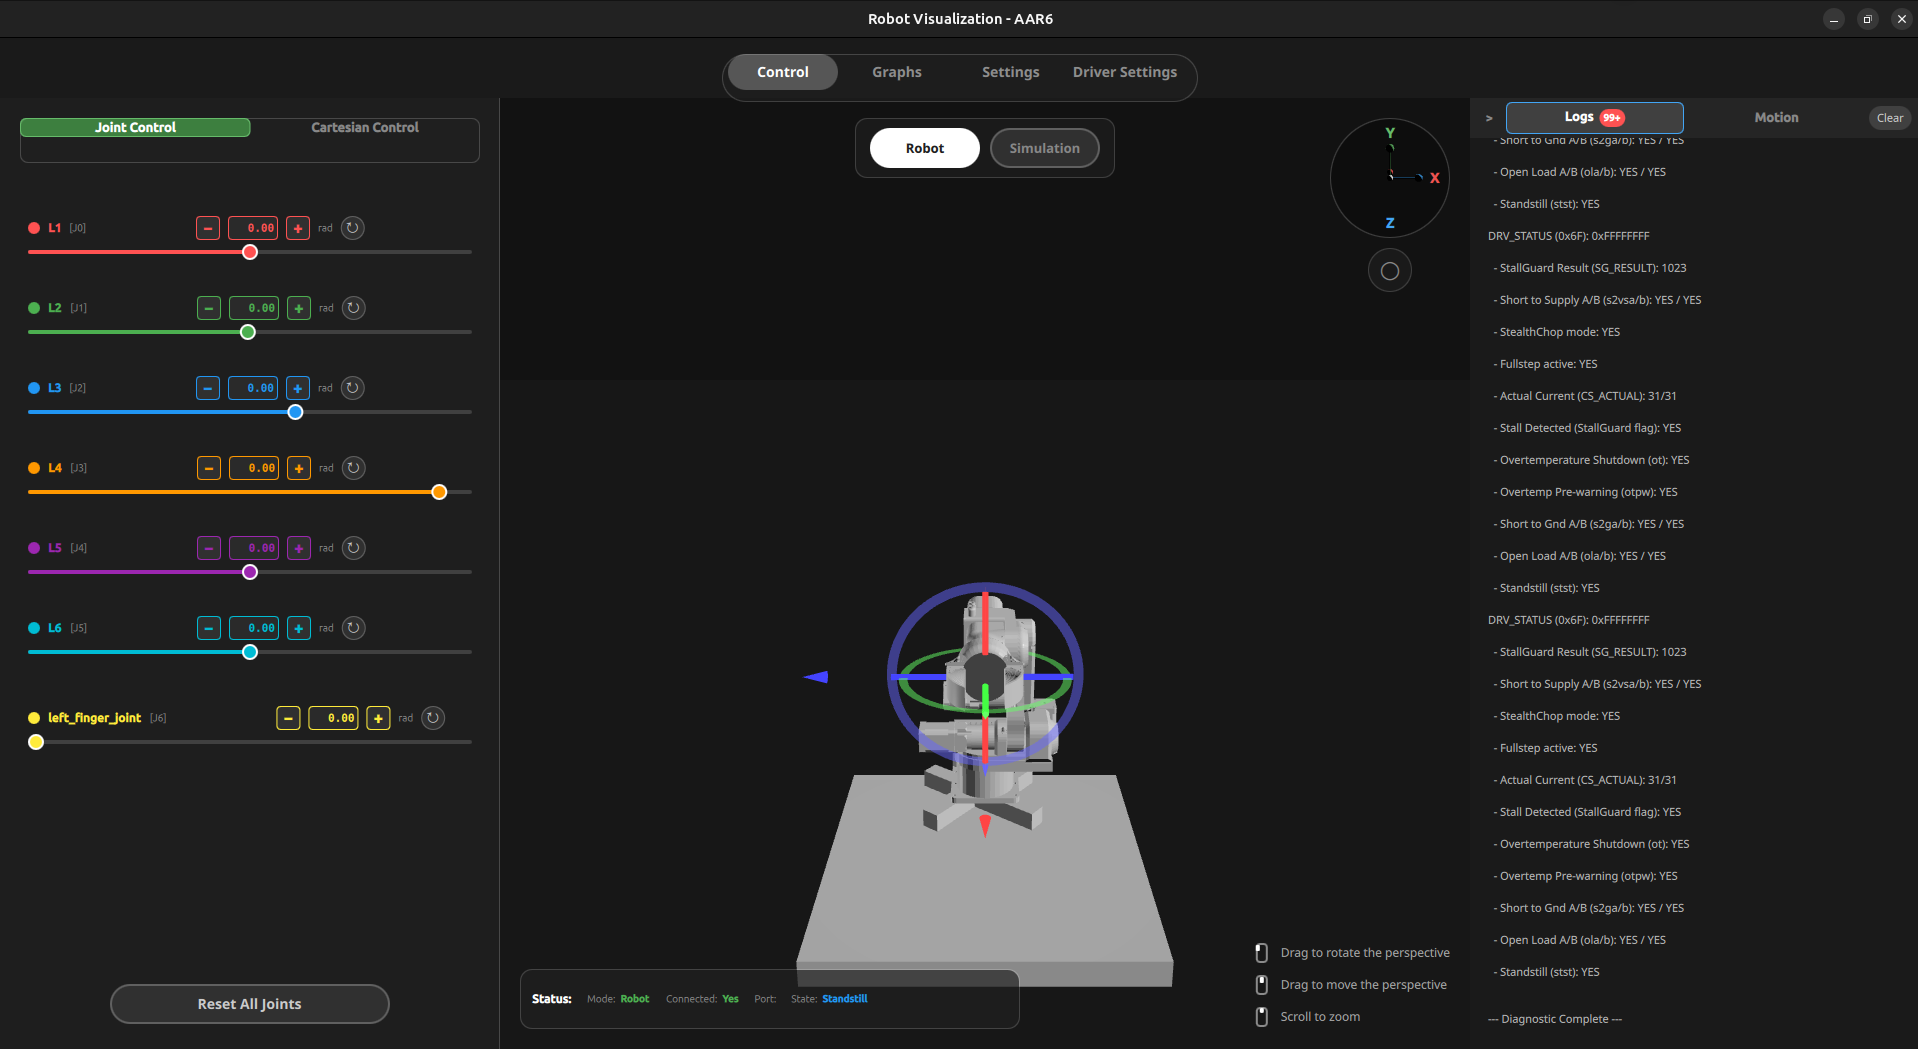
\includegraphics[width=0.8\textwidth]{images/viz_main.png}
    \caption{The Primary Control Interface showing the 3D robot model and control panels.}
    \label{fig:viz_main}
\end{figure}

\subsection{Connection and Initialization}

The software includes an automated hardware detection system. Upon startup, it scans the available serial ports to identify the custom MCU. Once detected, the system prompts the user to connect:

\begin{figure}[H]
    \centering
    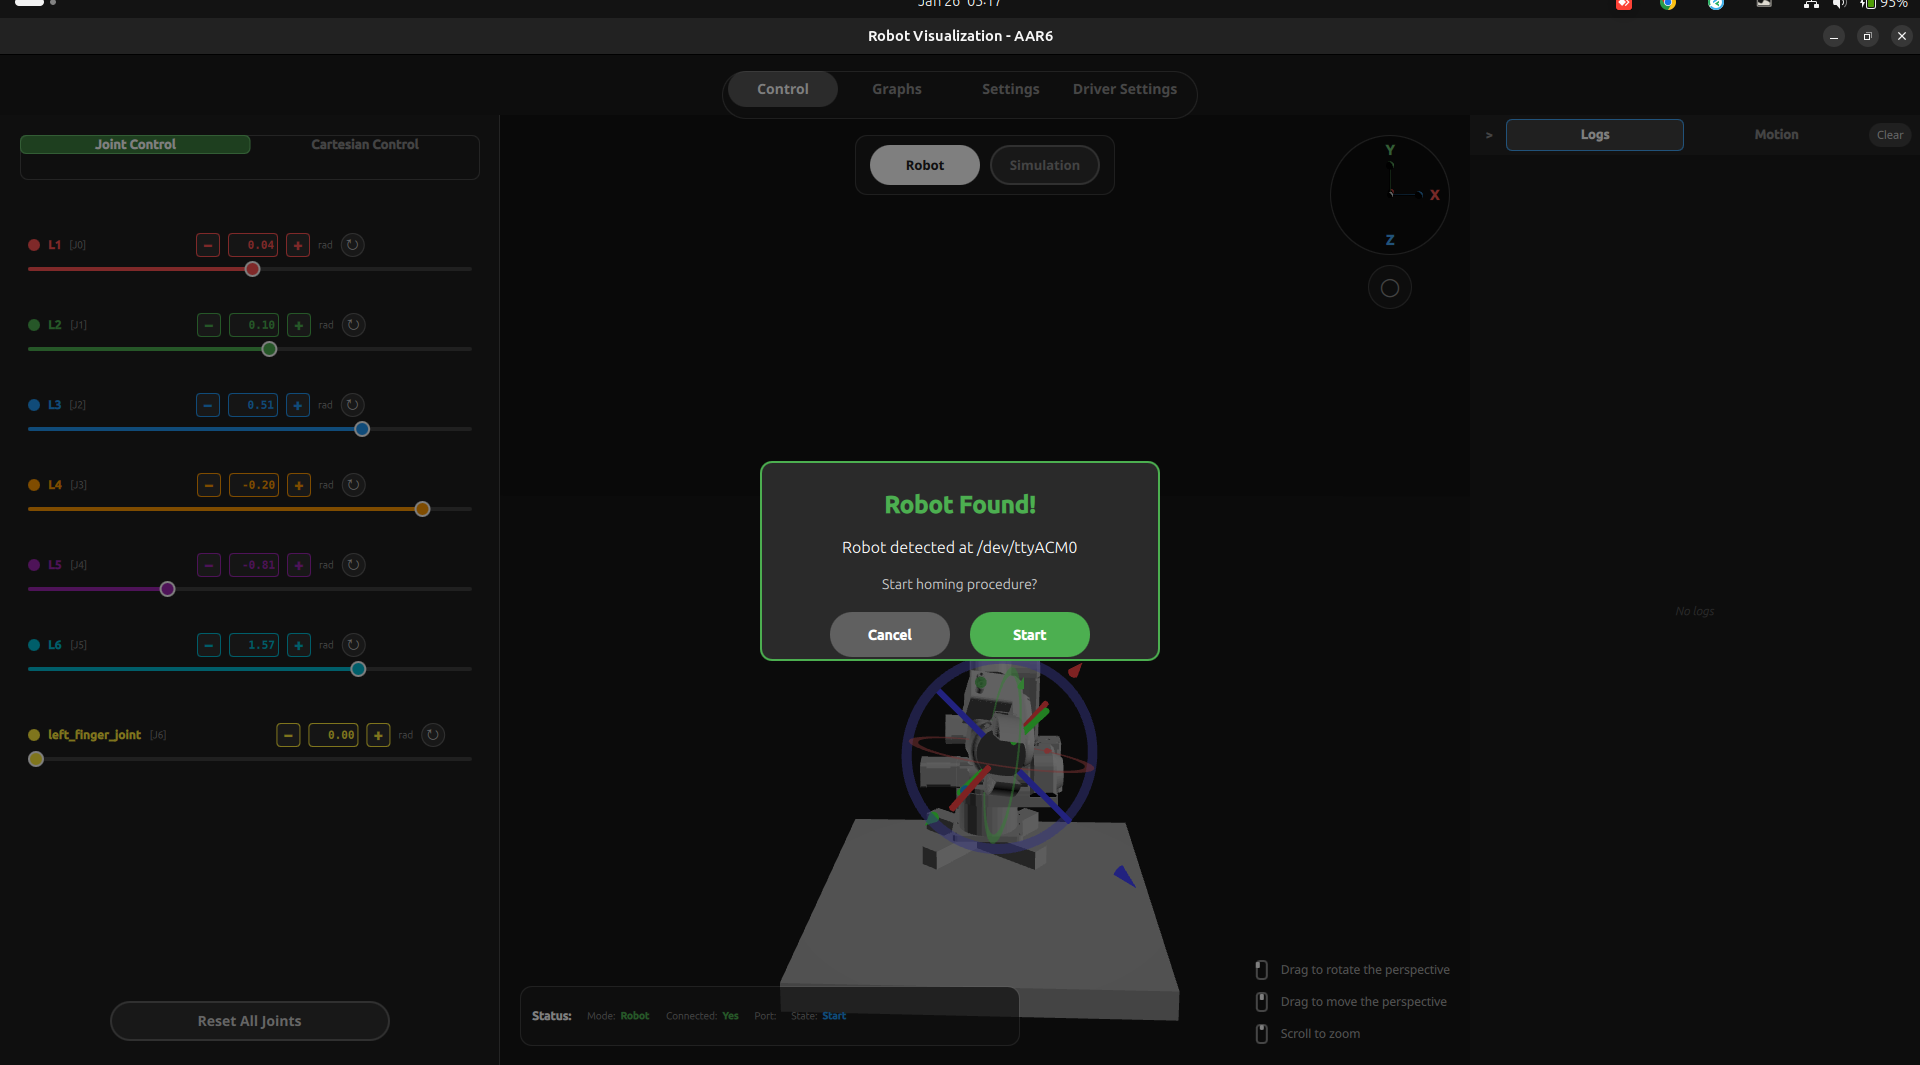
\includegraphics[width=0.6\textwidth]{images/viz_connect.png}
    \caption{The automated connection prompt and MCU detection status.}
    \label{fig:viz_connect}
\end{figure}

Upon successful connection, the software initiates a \textbf{Homing Sequence}. This ensures that the physical robot's joint positions are synchronized with the internal kinematic model, establishing a verified zero-frame for all subsequent motions.

\subsection{Control Modes and Input Methods}

The interface utilizes a Model-View-Controller (MVC) architecture where the \textbf{QML} layer handles the interactive 3D rendering and 2D controls, while the \textbf{C++} backend manages the thread-safe communication and IK computation.



Users can control the robot through several input modalities:

\begin{enumerate}
    \item \textbf{Cartesian Drag (3D Gizmo)}: 
    An interactive 3D transform gizmo is attached to the end-effector in the 3D view. Users can drag this gizmo to move the robot in real-time. The software solves the Differential QP-IK at high frequency, streaming smooth trajectories to the MCU.
    
    \begin{figure}[H]
        \centering
        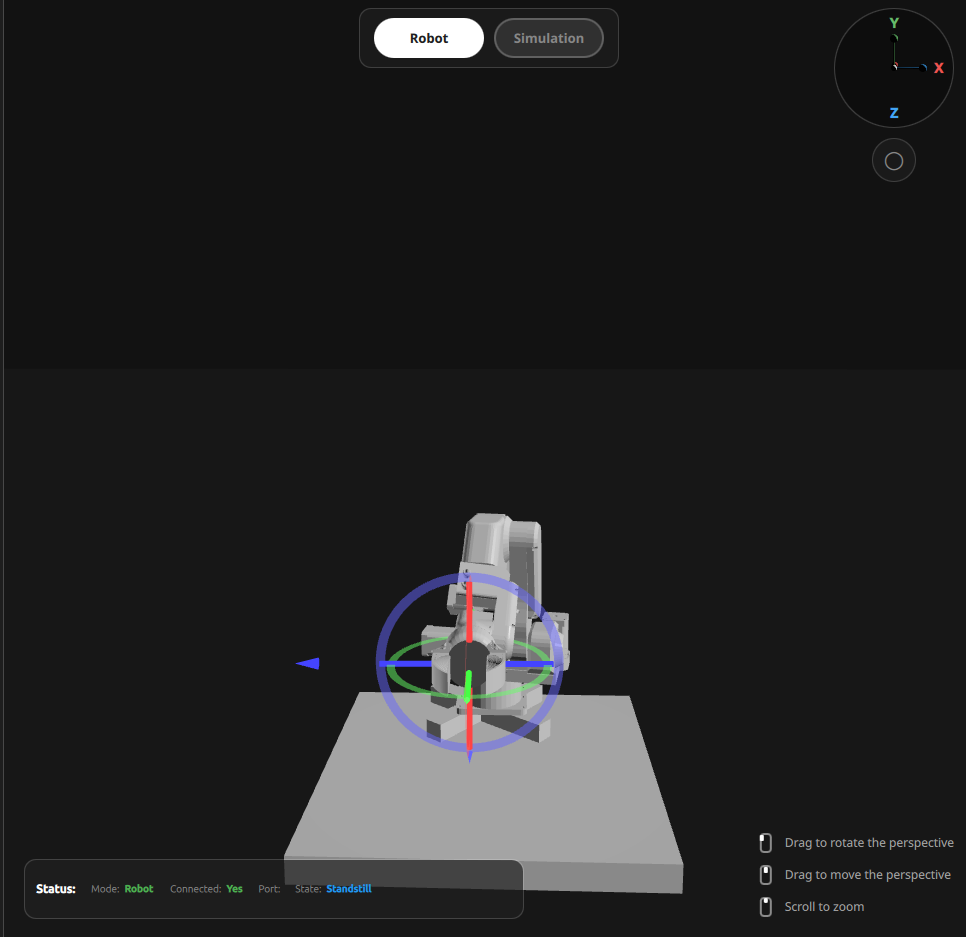
\includegraphics[width=0.7\textwidth]{images/vix_gizmo.png}
        \caption{Interactive 3D Gizmo for real-time Cartesian manipulation.}
        \label{fig:viz_gizmo}
    \end{figure}

    \item \textbf{Cartesian Command Panel}: 
    For precise numerical input, the Cartesian panel allows users to specify exact target coordinates and orientations. This is particularly useful for tasks requiring sub-millimeter precision that are difficult to achieve through 3D dragging alone.

    \begin{figure}[H]
        \centering
        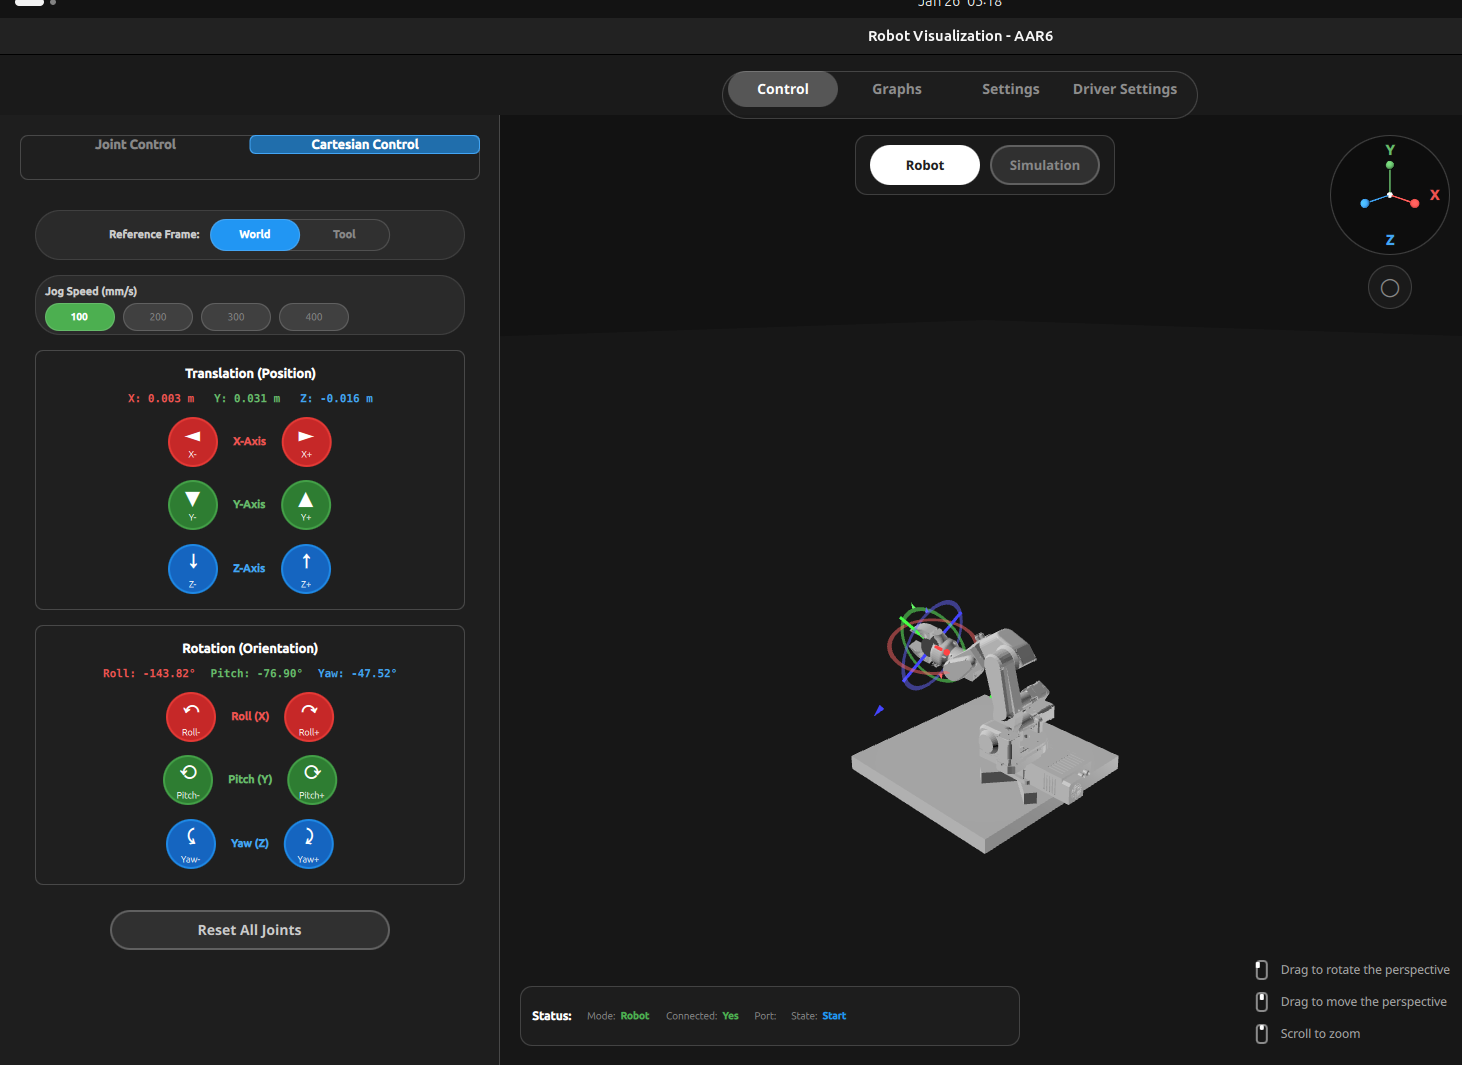
\includegraphics[width=0.7\textwidth]{images/viz_cartesian.png}
        \caption{Cartesian command and target coordinate panel.}
        \label{fig:viz_cartesian}
    \end{figure}

    \item \textbf{Joint-Space Sliders}: 
    Individual sliders permit direct manipulation of each joint angle (q1-q6). This is useful for manual configuration, diagnostic testing, and verification of individual actuator health.

    \begin{figure}[H]
        \centering
        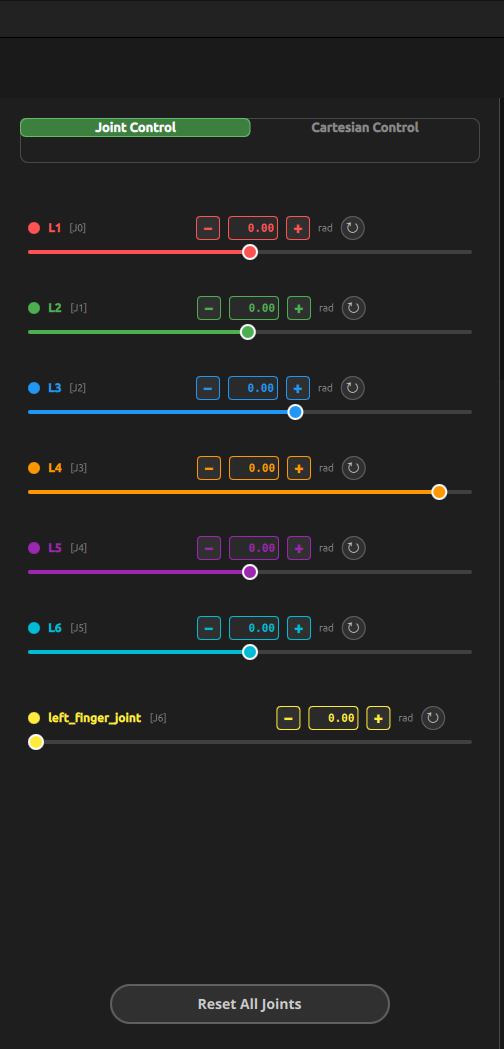
\includegraphics[width=0.6\textwidth]{images/viz_jointcontrol.png}
        \caption{Joint-space control interface (Sliders) and Cartesian command panel.}
        \label{fig:viz_controls}
    \end{figure}

    \item \textbf{Motion Planning and Waypoints}: 
    The software features a dedicated \textit{Motion Controller} and \textit{Panner}. Users can add specific pose waypoints to a sequence and play them back. The system interpolates between these points using the internal S-Curve engine to ensure smooth transitions.

    \begin{figure}[H]
        \centering
        \begin{minipage}{0.48\textwidth}
            \centering
            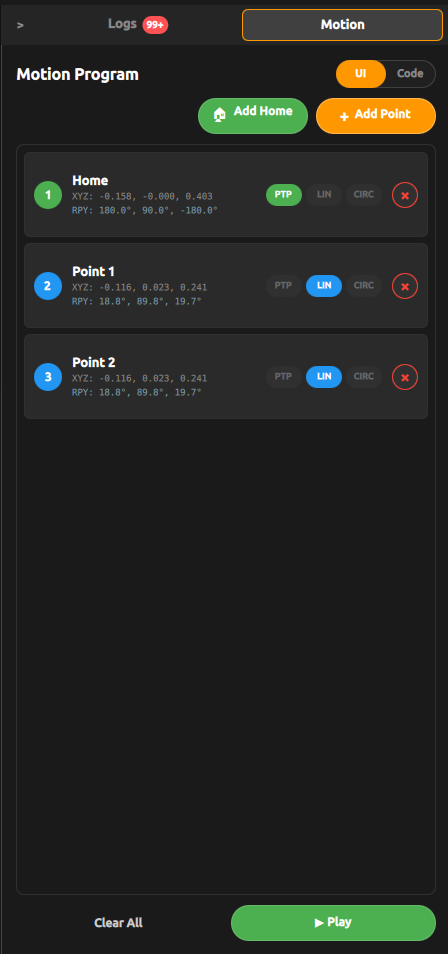
\includegraphics[width=\textwidth]{images/viz_motion_contoller.png}
            \caption{Motion waypoint sequence planner.}
        \end{minipage}\hfill
        \begin{minipage}{0.48\textwidth}
            \centering
            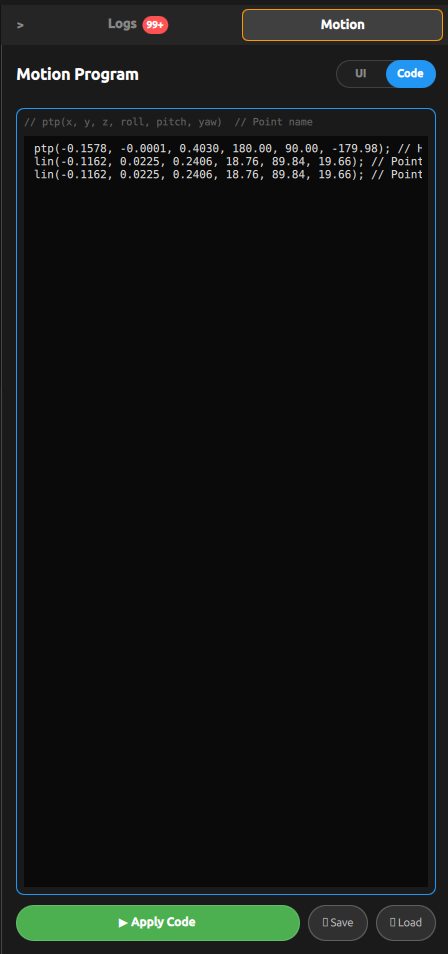
\includegraphics[width=\textwidth]{images/viz_montroller_code.png}
            \caption{Integrated scripting and code interface.}
        \end{minipage}
    \end{figure}

    \item \textbf{Scripting Interface}: 
    For complex task automation, users can write code directly within the interface to execute logic-based motion sequences, integrating sensor feedback or timed events.
\end{enumerate}

\subsection{System Telemetry and Visualization}

The 3D visualization is a mirror of the physical robot. As joint positions are streamed back from the MCU at 100\,Hz, the 3D model is updated via the Forward Kinematics engine, providing the user with an accurate representation of the robot's current state.

\begin{figure}[H]
    \centering
    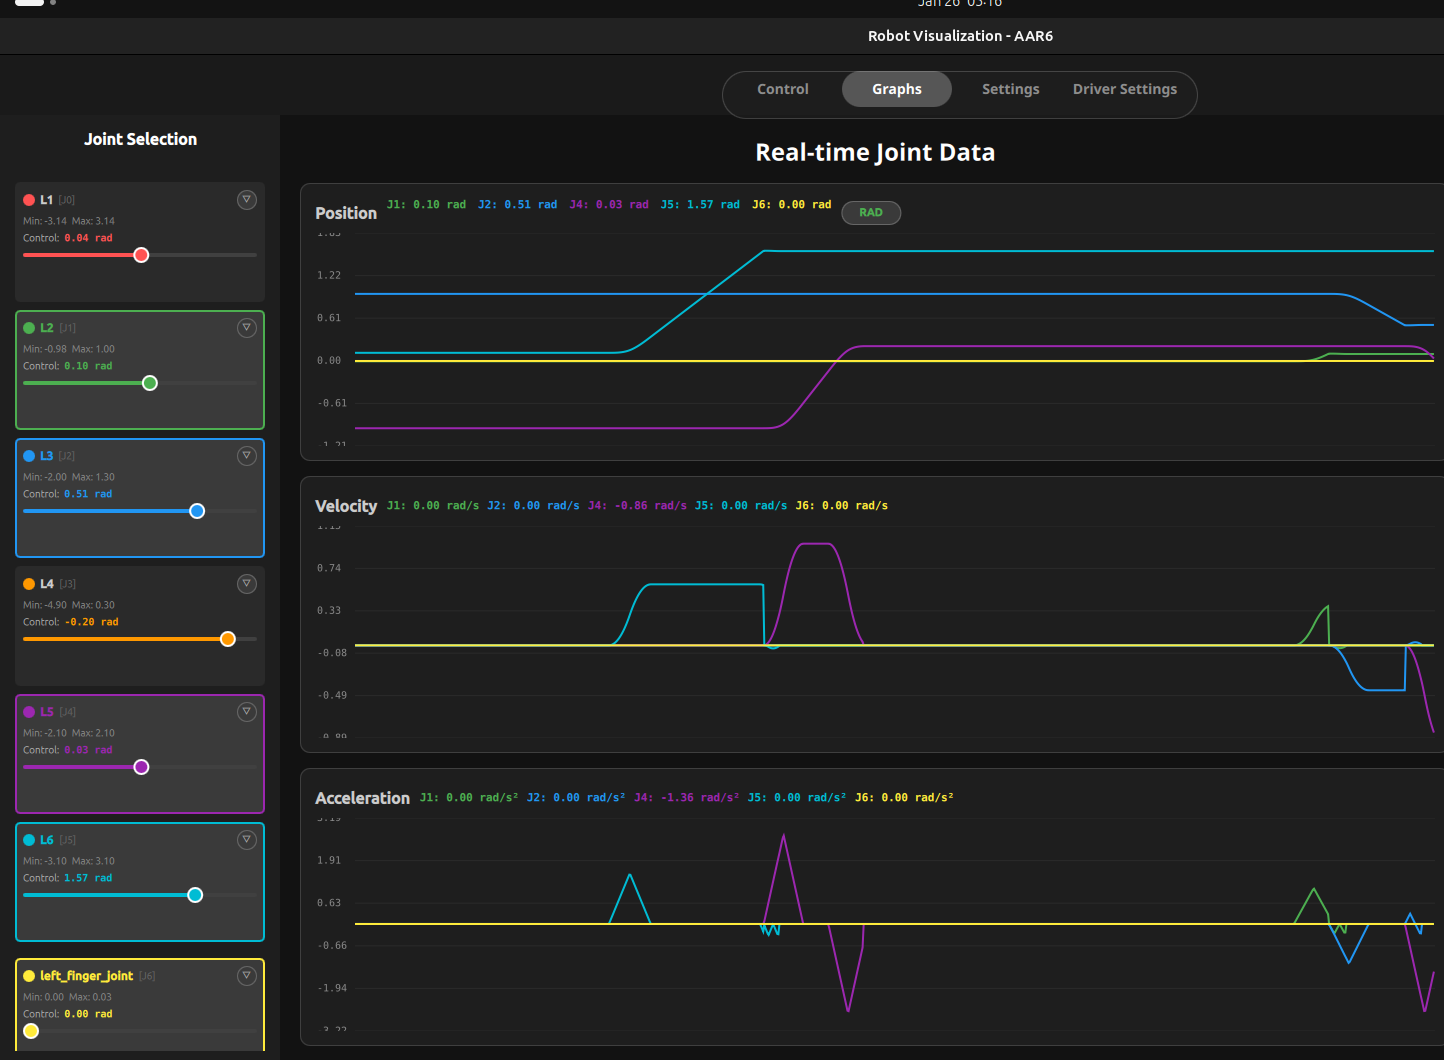
\includegraphics[width=0.8\textwidth]{images/viz-graphs.png}
    \caption{Real-time joint velocity and acceleration telemetry graphs.}
    \label{fig:viz_graphs}
\end{figure}

\section{Project Status: Limitations and Future Roadmap}

The current implementation provides a high-fidelity 6-DOF control system; however, technical constraints across hardware, control logic, and software frameworks define the roadmap for future development.

\subsection{Hardware and Connectivity}
\begin{itemize}
    \item \textbf{Actuator Driver Status (J3)}: The system is currently missing two primary drivers. A temporary "jerry-rigged" driver is currently in use for Joint 3 (J3); however, it is prone to thermal shutdowns due to temperature regulation issues and must be replaced. This failure mode was precipitated by high Back-EMF from J3, which destroyed two previous drivers. A high-quality, high-EMF-rated driver is required for stable long-term operation (\href{https://biqu.equipment/products/bigtreetech-tmc5160-v1-0-driver-spi-mode-silent-high-precision-stepstick-stepper-motor-driver-with-heatsink-for-skr-v1-3-gen-v1-4-reprap?variant=40301979598946}{TMC5160 Product Page}).
    \item \textbf{End-Effector (Gripper) Status}: The gripper is currently disconnected from the control loop. This is due to a combination of time constraints and the aforementioned driver failures, leaving insufficient functional drivers for complete integration.
    \item \textbf{Payload and Mass Distribution}: The NEMA-style stepper motor used for the gripper adds approximately 300\,g of dead weight at the end of the arm. This significantly reduces the effective payload capacity and increases the inertial load during high-acceleration maneuvers. 
    \item \textbf{Position Encoders (AS5600)}: The AS5600 magnetic encoders are currently not connected to the control loop. Once integrated, these will enable \textbf{Admittance Control} and adjustable arm stiffness. This hardware capability will allow for "lead-through" programming, where the user can teach the robot new paths simply by physically moving the arm.
\end{itemize}

\subsection{Kinematic and Dynamic Control}
\begin{itemize}
    \item \textbf{Collision Awareness}: The Differential IK solver does not natively account for self-collisions or obstacle avoidance. Future work involves adding Control Barrier Function (CBF) constraints to the QP formulation.
    \item \textbf{Full Dynamics Modeling}: The system is purely kinematic. Moving to a dynamic model (implementing gravity and inertia compensation) would significantly improve performance with heavy payloads.
    \item \textbf{Hybrid Singularities}: While SDLS handles mathematical singularities, the transition between discrete configuration branches (elbow flip) remains a focus for more advanced predictive "look-ahead" optimizations.
    \item \textbf{Jerk-Limited Motion}: The current controller provides smooth trajectories but is not inherently jerk-limited. This is because it solves a memoryless velocity-level QP. Achieving full jerk limiting would require either higher-order state constraints within the QP formulation or a dedicated time-domain filter applied as a post-processing stage.
\end{itemize}

\subsection{Software and Integration}
\begin{itemize}
    \item \textbf{Automatic Hardware Detection}: The current automatic MCU detection system is known to fail intermittently. Manual port selection or retry logic is sometimes required to establish a stable communication link.
    \item \textbf{Control Loop Performance}: The high-level control loop, while stable, has several identified paths for optimization. Reducing computational overhead in the IK solver and improving thread synchronization would enable higher streaming frequencies and lower control latency.
    \item \textbf{Code-Base Modularity}: Continual refactoring to separate the core kinematic solvers from the GUI logic will enhance the portability of the controller to other robotic platforms.
\end{itemize}


\begin{thebibliography}{9}
    \bibitem{buss} Buss, S. R., \& Kim, J. S. (2005). Selectively Damped Least Squares for Inverse Kinematics. \url{https://mathweb.ucsd.edu/~sbuss/ResearchWeb/ikmethods/SdlsPaper.pdf}
    \bibitem{ieee_sdls} Buss, S. R., \& Kim, J. S. (2005). A Selectively Damped Least Squares Method for Inverse Kinematics. \textit{IEEE/ASME Transactions on Mechatronics}, 10(3), 312--320. \url{https://ieeexplore.ieee.org/document/9757150}
    \bibitem{faverjon} Faverjon, B., \& Tournassoud, P. (1987). A local based approach for path planning of manipulators with a high number of degrees of freedom.
    \bibitem{mathworks} MathWorks. Manipulability index. Robotics System Toolbox. \url{https://www.mathworks.com/help/robotics/ref/manipulabilityindex.html}
    \bibitem{osqp} Stellato, B., Banjac, G., Goulart, P., Bemporad, A., \& Boyd, S. (2020). OSQP: an operator splitting solver for quadratic programs. \textit{Mathematical Programming Computation}, 12(4), 637--672.
    \bibitem{EAIK} Ostermeier, D., Külz, J., \& Althoff, M. (2025). Automatic Geometric Decomposition for Analytical Inverse Kinematics. \textit{IEEE Robotics and Automation Letters}, 10(10), 9964--9971.
    \bibitem{tmc5160_prod} BigTreeTech. TMC5160-V1.0 Stepper Motor Driver. Product Page. \url{https://biqu.equipment/products/bigtreetech-tmc5160-v1-0-driver-spi-mode-silent-high-precision-stepstick-stepper-motor-driver-with-heatsink-for-skr-v1-3-gen-v1-4-reprap}
\end{thebibliography}

%% ========================================
%% APPENDIX
%% ========================================

\appendix

\chapter{Source Code Repositories}
The source code for the various components of this project is hosted on GitHub.
\begin{itemize}
    \item \textbf{Control Board Firmware}: \url{[GitHub Link Placeholder]}
    \item \textbf{Robot Controller Software}: \url{[GitHub Link Placeholder]}
    \item \textbf{Visualization UI}: \url{[GitHub Link Placeholder]}
\end{itemize}


\end{document}
